




% Template for PLoS
% Version 1.0 January 2009
%
% To compile to pdf, run:
% latex plos.template
% bibtex plos.template
% latex plos.template
% latex plos.template
% dvipdf plos.template

\documentclass[10pt]{article}

% amsmath package, useful for mathematical formulas
\usepackage{amsmath}
% amssymb package, useful for mathematical symbols
\usepackage{amssymb}

% graphicx package, useful for including eps and pdf graphics
% include graphics with the command \inputgraphics
\usepackage{graphicx}
\usepackage{lscape}

% cite package, to clean up citations in the main text. Do not remove.
\usepackage{cite}

\usepackage{color} 

% Use doublespacing - comment out for single spacing
\usepackage{setspace} 
\doublespacing


% Text layout
\topmargin 0cm
\oddsidemargin 0.5cm
\evensidemargin 0.5cm
\textwidth 16cm 
\textheight 21cm

% Bold the 'Figure #' in the caption and separate it with a period
% Captions will be left justified
\usepackage[labelfont=bf,labelsep=period,justification=raggedright]{caption}

%load my own packages (not PLoS template)
\usepackage{textcomp, fixltx2e}
\usepackage{fullpage, lscape}
\usepackage{lineno}

% Use the PLoS provided bibtex style
\bibliographystyle{plos2009}

% Remove brackets from numbering in List of References
\makeatletter
\renewcommand{\@biblabel}[1]{\quad#1.}
\makeatother


% Leave date blank
\date{}

\pagestyle{myheadings}
%% ** EDIT HERE **


%% ** EDIT HERE **
%% PLEASE INCLUDE ALL MACROS BELOW

%% END MACROS SECTION

\usepackage{Sweave}
\begin{document}

% Title must be 150 characters or less
\begin{flushleft}
{\Large
\textbf{Controls of litter chemistry over early lignin decomposition in beech litter}
}
\\
% Insert Author names, affiliations and corresponding author email.
% Insert Author names, affiliations and corresponding author email.
Lukas Kohl$^{1}$, % $^{3,\ast}$
Wolfgang Wanek$^{1}$, 
Katharina Keiblinger$^{2,3}$, 
Sonja Leitner$^{1,3}$, 
Maria Mooshammer$^{1}$, 
Ieda H\"ammerle$^{1}$, 
Lucia Fuchslueger$^{1}$, 
J\"org Schnecker$^{1}$, 
Thomas Schneider$^{4,5}$
Sandra Moll$^{7}$
Markus Gorfer$^{7}$
Joseph Strauss$^{7}$
Katharina Riedel$^{4,6}$
Leo Eberl$^{4,5}$
Sophie Zechmeister-Boltenstern$^{2,3}$, 
Andreas Richter$^{1}$,
\\
\bf{1} Department of Chemical Ecology and Ecosystem Research, University of Vienna, Althanstrasse 14, A-1090 Vienna, Austria
\\
\bf{2} Federal Research and Training Centre for Forests, Natural Hazards and Landscape, Department of Soil Biology, Seckendorff-Gudent-Weg 8, A-1131 Vienna, Austria
\\
\bf{3} Current address: Institute for Soil Science, University of Natural Resources and Life Sciences, Peter Jordan-Stra\ss e 82, A-1180, Vienna, Austria
\\
\bf{4} Institute of Plant Biology, University of Zurich, Winterthurerstrasse 190, CH-8057, Zurich, Switzerland
\\
\bf{5} Current address: Institute of Plant Biology, University of Zurich, Zollikerstrasse 107, CH-8008, Zurich, Switzerland
\\
\bf{6} Current address: Institute of Microbiology, Ernst-Moritz-Arndt University of Greifswald, Friedrich-Ludwig-Jahn-Strasse 15, D-17487 Greifswald, Germany
\\
\bf{7} Current address: Department of Applied Genetics and Cell Biology, University of Natural Resources and Life Sciences, Muthga\ss e 18, A-1190, Vienna, Austria

$\ast$ E-mail: Corresponding author@institute.edu
\end{flushleft}

\newpage
% Please keep the abstract between 250 and 300 words
\section*{Abstract}

Lignin is a major component of plant litter and is considered highly resistant to decomposition. Polymeric carbohydrates, in contrast, are more easily accessible carbon sources. We studied the decomposition rates of these two compound classes, to which extent they are controlled by litter C:N:P stoichiometry, and whether this control changes over time. Therefore, we conducted a 15-months mesocosm experiment under controlled climatic conditions, comparing beech litter of different N and P contents, which was sterilized and re-inoculated with a litter/topsoil mixture from one of the sites to ensure identical microbial communities at the start of the experiment. Lignin and carbohydrate decomposition rates were calculated for 2 periods (0-6 months and 6-15 months) by pyrolysis-GC/MS.

Positive correlations of carbohydrate decomposition rates with litter N content were found during the entire experiment. Lignin decomposition rates during the initial period were highly variable and negatively correlated to litter P content and positively correlated to the microbial P demand (C:P\textsubscript{litter}/C:P\textsubscript{microbial}). During the later stage, both lignin and carbohydrate decomposition loss were positively correlated to N contents and respiration. Initial lignin decomposition rates were highest in litter with low fungi:bacteria ratios, which occurred in N and P poor litter.

Our results showed that a substantial amount of lignin can be degraded during early decomposition. In the present study, early lignin decomposition was coupled to low N and P availability, and the establishment of K-strategist microorganisms. However, early lignin decomposition rates did not depend on fungi, which are commonly assumed to mediate lignin decomposition, or stoichiometric conditions that favor fungal growth. 

\linenumbers %not from the template: start line numbers here.
\newpage%not in original layout
\section*{Introduction}

Plant litter is quantitatively dominated by macromolecular compounds. In foliar litter, lignin and carbohydrate polymers together make up 40-60\% of litter dry mass \cite{Berg2008}, while leachable substances ("DOM") account for only 1.5-6\% \cite{Don2005}. The breakdown of these high molecular weight compounds into smaller molecules accessible to microbes is mediated by extracellular enzymes and considered rate limiting for decomposition processes \cite{Sinsabaugh2010}

Litter decomposition models generally follow the concept that organic compounds in litter form up to three independent pools of increasing recalcitrance, i.e. (1) soluble compounds, (2) cellulose and hemi-celluloses, and (3) lignin and waxes (cutin and suberin). Soluble compounds are most accessible to microbes and are usually consumed first, followed by regular polymers, such as cellulose. Lignin is not degraded until accumulated to a certain, critical level when it inhibits the degradation of less recalcitrant compounds\cite{Berg1980, Couteaux1995, Moorhead2006, Adair2008}. These pools are usually quantified by gravimetric determination of the amount of cellulose, hemi-celluloses and lignins after sequential extractions with selective solvents. These methods were repeatedly criticized for being unspecific for lignin determination \cite{Hatfield2005}. When analyzed with alternative methods (NMR, CuO-oxidation, Pyrolysis-GC/MS), extracted lignin fractions were shown to contain also many other substances \cite{Preston1997}.

Recent studies based on more specific methods to determine litter lignin contents question the assumed intrinsic recalcitrance of lignin. Isotope labeling experiments with soils and litter/soil mixtures, undertaken both in-situ and under controlled conditions,  revealed mean residence times of lignin in soils are in the range of 10-50 years, much less then expected and shorter than that of bulk soil organic matter or many other carbon compounds \cite{Amelung2008, Thevenot2010a, Bol2009}. Also, the capability to degrade lignin was demonstrated for several bacterial taxa in addition to fungi \cite{Bugg2011}.

For leaf litter, lignin depletion even at early stages of decomposition and lignin decomposition rates that decreased during decomposition were recently reported by Klotzb\"{u}cher and colleagues \cite{Klotzbucher2011}. Based on these results, they proposed a new concept for lignin degradation in which fastest lignin degradation occurs during early litter decomposition when the availability of labile carbon sources is high. Lignin decomposition during late decomposition, in contrast, is limited by the availability of easily assimilated C and therefore slowes down. Additionally, the decomposition of lignin may also be dependent on the nutrient content of the litter and thus the status of the microbial community. During radical polymerization, significant amounts of cellulose and protein are incorporated into lignin structures \cite{Achyuthan2010}. In isolated lignin fractions from fresh beech litter, N contents twice as high as in bulk litter were found \cite{Dyckmans2002}. It was therefore argued that, while yielding little C and energy, lignin decomposition makes protein accessible to decomposers that is occluded in plant cell walls, and that lignin decomposition is therefore not driven by C but by the N demand of the microbial community ("Nitrogen mining theory", \cite{Craine2007}). 

In favor of the N mining theory, fertilization experiments indicated N exerts an important control on lignin degradation: N addition increased mass loss rates in low-lignin litter while slowing down decomposition in lignin-rich litter \cite{Knorr2005} and decreased the activity of lignolytic enzymes in forest soils \cite{Sinsabaugh2010}. Moreover, cellulose triggered a stronger priming effect in fertilized than in unfertilized soils indicating that the mineralization of recalcitrant carbon may be controlled by an interaction of N and labile C availability \cite{Fontaine2011}.

Addition of N has a different effect on litter decomposition than varying N levels in the litter \cite{Talbot2011}. This is due to the fact that leaf litter N is stored in protein and lignin structures and not directly available to microorganisms, while fertilizer N is added in the form of readily available inorganic N (ammonium, nitrate or urea). N-fertilization experiments can thus simulate increased N-deposition rates but not the effect of litter N on decomposition processes.

Our study therefore aimed at analyzing the effect of variations in beech litter nutrient (N and P) content and stoichiometry (C:N and N:P ratios) on lignin and carbohydrate decomposition rates. Towards this end, we followed the breakdown of lignin and polymeric carbohydrates by pyrolysis-GC/MS (pyr-GC/MS) during a mesocosm experiment under constant environmental conditions over a period of 15 month. In order to exclude effects resulting from different initial microbial communities, we sterilized beech litter samples from 4 different locations in Austria and re-inoculated them prior to the experiment with an litter/top-soil inoculum from one of the sites.  
[one sentence on metaproteome/qPCR here]

We addressed the following questions in our study:

(1) Is lignin decomposition delayed until late decomposition stages or are significant amounts of lignin already degraded during early litter decomposition, and if the timing of lignin decomposition depended on litter stoichiometry? We hypothesized, that ligin decomposition is initially slower in litter with a narrow C:N ratio (higher availability of assimilable nitrogen), than in litter with a high C:N ratio.

(2) Are high lignin degradation rates related to a higher fungal activity? We hypothesized that wider C:N and C:P ratios favor lignin degradation by fungi while narrow C:N and C:P ratios favor carbohydrate degradation by bacteria. 
% Results and Discussion can be combined.
\section*{Results}
\subsection*{Initial litter chemistry}
Initital litter chemistry (14 days after incubation) is presented in table \ref{initstoech}. C:N ratios between 41:1 and 58:1 and C:P ratios between 700:1 and 1300:1 were found, N:P ratios ranged between 15:1 and 30:1. No significant changes occurred during litter incubation except a slight decrease of the C:N ratio (41.8:1 to 37.4:1) found in the most active litter type (SW) after 15 month. Fe concentrations were more than twice as high for OS (approx. 450 ppm) than for other litter types (approx. 200 ppm). Litter Mn also was highly variable between litter types, ranging between 170 and 2130 ppm. Changes of micro-nutrient concentrations during litter incubation were significant, but in all cases \textless 15\% of the initial concentration. In initial litter, lignin accounted for 28.9-31.2\% and carbohydrates for 25.9-29.2\% of the total peak area of all pyrolysis products.

\subsection*{Mass loss, respiration and extractable organic carbon}

Litter mass loss was not significant after 2 weeks and 3 months, and significant for 2 litter types after 6 months. After 15 months, litter mass loss was significant for all litter types, ranged between 5 and 12 \% of the initial dry mass, and was strongly correlated to litter N content (R=0.794, p\textless 0.001). Detailed results were reported by \cite{Mooshammer2011}.

Highest respiration rates were measured at the first measurement after 14 days incubation (150-350 \textmu g CO$_2$-C d$^{-1}$ g$^{-1}$ litter-C), which dropped to 75 to 100 \textmu g CO$_2$-C d$^{-1}$ g$^{-1}$ litter-C after 3 months. After 6 and 15 months, respiration rates for AK and OS further decreased, while SW and KL showed a second maximum in respiration after 6 months days (fig \ref{fig:enz}). Accumulated respiration was correlated to litter mass loss (r=0.738, p\textless 0.001, n=20).%\footnote{or r=0.961, p=0.038, n=4 if means are compared are used.}

Soluble organic carbon concentrations decreased between the first three harvests (14 days to 6 months), and strongly increased to 15 months (from 0.1 to 0.7 mg C g$^{-1}$  d.w. to 1.5 to 4 mg C g$^{-1}$ d.w. after 15 months, fig. \ref{fig:enz}). After 14 days and 3 months, the highest soluble organic C concentration was found in SW litter followed by AK. Soluble organic C concentrations were weakly correlated with litter N content after 14 days (r=0.69, p\textless 0.001) and after 3 months (r = 0.65, p\textless 0.01), but were strictly correlated after 6 months (r=0.85, p\textless 0.001) and 15 months (r=0.90, p\textless 0.001).

%\begin{figure*}[t]
%\vspace*{2mm}
%\begin{center}
%\setkeys{Gin}{width=0.5\textwidth}
%<<doc, echo=F, results=hide, fig=T, height=7, width=7>>=
%timeseries(alldata$DOC/1000, alldata$days, alldata$Litter, pch=pch, pt.bg=colscale,  xlab="Incubation (days)", ylab="mg C g-1 d.w.", main="Extractable carbon", lwd=2)
%legend("bottomright", pt.bg=colscale, pch=pch, typlev, lty=1, lwd=2)
%@
%\end{center}
%\caption{Extractable organic carbon. Error bars indicate standard errors (n=5).}
%\label{fig:doc}
%\end{figure*}

\subsubsection*{Potential enzyme activities}
Potential extracellular enzyme activities were correlated with litter N, respiration and other decomposition processes (all R\textgreater 0.8, p\textless 0.001). Cellulase activity increased from first harvest onwards to 15 months, with a small depression after 6 months (Fig. \ref{fig:enz}), phenoloxidase and peroxidase activities reached their maximum after between 3 and 6 months (fig. \ref{fig:enz}). For all enzymes and at all time points, SW showed the highest and AK the lowest activity. Differences between these two sites were more pronounced in cellulase activity (SW 10x higher than AK) than in oxidative enzymes (4x higher). Conversely, the phenoloxidase/cellulase ratio was highest for AK and lowest for SW at all time points and decreased during litter decomposition. This indicates that microbial communities in AK litter invested more energy and nitrogen into degrading lignin and less into degrading carbohydrates than in litter from other sites. (fig. \ref{fig:enz}).

\subsubsection*{Microbial biomass abundance and community composition}
Microbial biomass contents ranged from 0.5 to 6 mg C g$^{-1}$ d.w., 0.05 to 5.5 mg N g$^{-1}$ d.w. and 0.05 to 3.5 mg P g$^{-1}$ litter d.w (fig. \ref{fig:mb}). In KL and OS microbial biomass buildup reached a plateau after 3 months, AK and SW showed further microbial biomass growth reaching a maximum of microbial C and N contents after 6 months (AK also for P). Microbial C:N ratios ranged between 6 and 18, C:P ratios between 8 and 35, and N:P ratios between 0.5 and 3.5 (fig. \ref{fig:mb}).

Litter microbial biomass was stoichiometrically homeostatic during the first 6 months (no or marginally negative correlations between microbial C:N:P and litter C:N:P, see also \cite{Mooshammer2011}), but after 15 months (microbial C:N:P ratios were significantly correlated to resource stoichiometry: R=0.53-0.64, all p\textless 0.002), when the homeostatic regulation coefficients \cite{Sterner2002} H\textsubscript{C:P}=1.68, H\textsubscript{C:N}=2.01, and H\textsubscript{N:P}=2.29 were found. Microbial C:N ratios were tightly constrained after 3 months (14.5 to 18.2) and 6 months (6.9 to 9.0), but significantly different between the two time points. Microbial C:P and N:P ratios were less constrained, with the highest variance between litter from different sites after 3 months incubation (fig. \ref{fig:mb}).

Fungi/bacteria ratios derived from metaproteomics data of the litter (one replicate per litter type and harvest) were highest after 14 days (5 to 12) and decreased during litter decomposition (1.7 to 3 after 15 months). The large differences in fungi/bacteria ratios between litter types decreased during decomposition. Fungal proteins were dominant in all litter types at all stages, but most prominent in SW and least pronounced in  AK. The fungi/bacteria ratios were negatively correlated to the ratios of lignin/cellulose decomposition and to LCI change during the first 6 months. In contrast, lignin decomposition rates were positively correlated with fungi/bacteria ratios after 15 months but not to the ratios of lignin/cellulose decomposition (fig. \ref{fig:f2b}). In addition, fungi: bacteria ratios were measured on a DNA basis (qPCR) the results showing a similar pattern between litter types and harvests but with a much larger fungal DNA dominance (ratios between 10-180). Fungi/bacteria ratios were highly correlated between protein- and DNA-based estimates (r=0.801, p\textless 0.001, with log-transformed qPCR ratios).

\subsection*{Pyrolysis-GC/MS and Lignin content}
In total 128 pyrolysis products were detected, quantified, identified and assigned to their origin (\ref{tab:phprod} -\ref{tab:nprod}). We found only minor changes in the relative concentration of litter pyrolysis products during decomposition, and differences between sites were small but well preserved during decomposition. However, the high precision and reproducibility of pyrolysis GC/MS analysis of litter allowed tracing small changes in lignin and carbohydrate abundance during decomposition. Lignin-derived compounds made up between 29 and 31 \% relative peak area (TIC) in initial litter, and increased by up to 3 \% over the first 6 months. Carbohydrate-derived pyrolysis products accounted for 26 to 29 \% in initial litter and decreased by up to 2.6 \% during litter decomposition. The pyrolysis-based LCI index  showed a small range between 0.517 and 0.533 initially (Fig. 4). During decomposition, LCI increased by up to 9 \% of the initial value, with SW showing the highest increase while in AK LCI decreased. The changes in LCI almost completely occurred over the first 6 months, with insignificant changes thereafter (fig. \ref{fig:lci}).

During the first 6 months of litter decomposition, between one and 6 \% of the initial lignin pool and between 4 and 17\% of the initial carbohydrate pool were degraded (Fig. \ref{fig:degr}). Lignin decomposition was highest in AK and KL litter, while KL, OS and SW decomposed carbohydrates fastest. Lignin preference values (\% lignin decomposed/\%carbohydrates decomposed) were lowest in SW and highest in AK litter (Figure 5). In AK litter, lignin macromolecules were 50 \% more likely to be decomposed than carbohydrates, while in SW litter carbohydrates were 10 times more likely to be decomposed (fig. \ref{fig:degr}). Between 6 and 15 months, no further accumulation of lignin occurred, lignin and carbohydrates were both degraded at the same rates and their relative concentrations remained constant (fig. \ref{fig:degr}).

\subsection*{Correlations between lignin and carbohydrate decomposition and litter chemistry, microbial community and decomposition processes}

Relationships between lignin and carbohydrate degradation, litter chemistry, microbial biomass and decomposition processes were tested after 6 and 15 months (tables \ref{corrtable} and \ref{corrtable2}) including data presented by \cite{Mooshammer2011} and \cite{Leitner2011}. After 6 months, we found that the ratio of lignin/cellulose degradation was positively correlated with the ratio of phenoloxidase/cellulase (R=0.599, p=0.005) and peroxidase/cellulase (R=0.734 p\textless 0.001, table \ref{corrtable}). Carbohydrate decomposition was positively correlated with litter N content, and negatively with litter C:N ratios and litter-microbial C:N imbalances. In contrast, lignin decomposition was negatively correlated to litter P, but positively with litter C:P and N:P ratios, and litter-microbial C:P and N:P imbalances (fig. \ref{fig:cor1}). After 15 months, the ratio of lignin/carbohydrate decomposition was not related to stoichiometry or elemental composition any more. Most interestingly, lignin and carbohydrate decomposition exhibited the same controls, being positively correlated to soluble organic C, litter N and litter P (table \ref{corrtable2}). Mass loss and accumulated respiration were positively correlated to lignin and carbohydrate decomposition (table \ref{corrtable2}), a pattern that we did not find for lignin decomposition in the early decomposition phase (table \ref{corrtable}).

\section*{Discussion}

Our experimental approach allowed us to single out the effects of litter quality on the microbial decomposer community as well as decomposition processes, while excluding effects of fauna, climate and the initial microbial community. By exploiting intra-specific differences in beech litter stoichiometry, we were able to minimize differences in the chemical composition of initial litter (e.g. similar lignin and cellulose content, table \ref{initstoech}), while exploring the effect of litter nutrient contents on lignin and carbohydrate decomposition. Therefore, we can attribute different rates of carbohydrate and lignin decomposition to the intrinsic qualities of litter collected at different sites, i.e. elemental and stoichiometric composition.

Contradicting the traditional concepts of litter decomposition, our results demonstrate that relevant but variable amounts of lignin were degraded during the first 6 months of incubation. During this early stage, lignin decomposition rates depended on litter quality (P) and ranged from non-significant to degradation rates similar to bulk carbon mineralization rates (i.e. no discrimination against lignin). We can therefore confirm that early lignin decomposition rates are by far underestimated, as recently proposed by \cite{Klotzbucher2011}, based on a complementary analytic approach. Unlike them, we found no decreases but constant or increasing lignin decomposition rates during litter decomposition over 15 months. Additionally, we found a marked change in the controls of lignin decomposition during this period. While carbohydrate and lignin decomposition were differently controlled by litter chemistry (N versus P) during the first 6 months, these litter components were decomposed at similar rates thereafter and decomposition rates were only related to litter N availability.

Differences in initial lignin contents were marginal (29-31 \% relative peak area), and lignin contents of sites with high initial lignin decomposition rates were not higher than that of sites with low rates. Therefore, differences in early lignin decomposition did not result from high or low lignin contents as is suggested by traditional litter decomposition models. Low lignin decomposition rates were also not caused by a lack of Mn or Fe, the metals being important cofactors of oxidative lignin decay, which were suggested to be rate limiting during late lignin decomposition \cite{Berg2008}. While Mn and Fe concentrations strongly varied between litter collected at different sites, Mn and Fe concentrations were lowest in the litter with highest lignin decomposition rates (AK, see Table \ref{initstoech}). Low contents of these elements would explain decreased but not enhanced lignin decomposition. Moreover, soluble organic C was suggested to be limiting for lignin decomposition since the process of lignin decomposition does not generate enough energy for survival of lignin decomposers \cite{Klotzbucher2011}. Soluble organic C apparently did not control lignin decomposition since we found highest concentrations in the two litter types that showed the highest and the lowest lignin decomposition rates.

We found strong evidence that litter C:N:P stoichiometry and litter element concentrations exerted a major control on the extent of lignin decomposition during the initial decomposition phase. Carbohydrate decomposition was positively correlated with litter N contents and negatively to litter C:N ratios, as were the majority of decomposition processes (mass loss, respiration, potential extracellular enzymatic activities). In contrast, lignin decomposition rates were positively correlated with litter C:P ratios and negatively with dissolved and total litter P. The relationship was strongest when lignin decomposition rates were compared to litter-microbe C:P imbalances, i.e. the greater the imbalance between resource and consumer C:P became (greater P limitation) the lower lignin decomposition rates became.

Cultivation studies showed that lignin decomposition by fungi is triggered by nitrogen starvation, and that lignin does not provide sufficient energy to maintain the decomposer's metabolism without the use of other organic C i.e. energy sources \cite{Janshekar1988}. Moreover, lignin decomposition was found in wild-type \emph{A. thaliana} litter containing abundant cellulose as a C source, but not in a low-cellulose mutant during a 12-month incubation experiment in a boreal forest \cite{Talbot2011}. In the N- and P-(co-)limited situation commonly encountered during early litter decomposition, we may speculate that lignin is degraded to access additional nutrients (mainly N) or to use a C surplus by decomposing a less C efficient but nutrient enriched substrate (nutrient mining hypothesis). However, a stimulation of lignin decomposition by low P availability or microbial P limitation, as indicated by the strong negative correlations to P pools that we found, has not been reported yet. Though lignified materials have been reported to be N-rich and decomposition of these materials may therefore enhance N supply to microbial communities, lignins are not expected to contain quantitative important amounts of P.

In order to decompose litter lignin and carbohydrates, microbial decomposers rely on the production and excretion of hydrolytic and oxidative extracellular enzymes. While the absolute amounts, in which these enzymes are produced, were largely controlled by N availability, the ratio in which they were produced was strongly related to differences in the ratio of cellulose/lignin decomposition. \cite{Talbot2011} suggested that lignin decomposition comprises a strategy of slow-growing microbes to evade competition through colonizing more lignin-rich and nutrient-poor substrates. Indeed we found lignin decomposition in low quality litter (low N and P) with microbial communities that were subject to large imbalances in C:N and C:P between resource and consumer, pointing to N and P limitation or high N and P uns efficiency of these communities. Low P availability may limit fast growth of microbial populations and select for slow-growing lignin-degrading microbes during early decomposition and provide K-strategists (slow growing on recalcitrant carbon) an advantage over r strategists (fast growing on labile carbon). Indeed we found that lignin decomposition was highest in litter, where resource C:P and N:P were highest, i.e. low P supply may have limited microbial growth generally or the establishment of r strategists in particular.

While the mode of negative P regulation on lignin decomposition remains unknown, we found differences in the composition of the microbial decomposer communities on litter with fast and slow lignin decomposition. Unlike predicted by ecological stoichiometry theory, not bacteria but fungi were more successful in colonizing high N and high P litter during initial decomposition. Fungi colonized litter faster than bacteria and therefore dominated early litter decomposition, however the fungi: bacteria ratios decreased over the entire incubation period pointing to increasing population sizes of bacteria with time. Fungi-rich communities more efficiently used high litter N to produce extracellular enzymes that degrade carbohydrates immediately after inoculation (fungi: bacteria ratios were correlated to litter N 14 days after inoculation) and high litter P to build up microbial biomass on a longer time scale (fungi: bacteria ratios were correlated to litter P after 6 months). Interestingly, low F:B communities (AK) were more active in decomposing lignin than those being dominated by fungi. This does not necessarily indicate that bacteria play the key role in lignin decomposition, though bacteria were also reported to produce oxidative enzymes that can decompose lignified materials in litter \cite{Bugg2011}. However, decreases in fungi:bacteria ratios may be superimposed on the increase of smaller subpopulations of e.g. fungi that are key mediators of lignin decomposition, or alternatively general increases in the size of microbial communities with declining fungi/bacteria ratios may as well mask stable fungal populations when  bacterial abundance increases. The fungal communities were dominated by Ascomycetes, with smaller contributions by Basidiomycetes. It is particularly the latter, Basidiomycetes, that catalyze the cellulolytic and lignolytic decomposition of dead plant material, however they comprised less that 5\% of the fungal protein ensemble. The bacterial community in contrast was dominated by Proteobacteria (mainly $\gamma$, declining, and $\alpha$- and $\beta$-Proteobacteria, increasing with litter decomposition), Actinobacteria and Bacteroidetes both of which strongly increased with time. Actinobacteria are also known as important decomposers of plant detritus, with the potential to excrete oxidative enzymes and being oligotrophic, and Bacteroidetes also excrete a broad range of hydrolytic enzymes targeting cellulose and other polymers. Since the metaproteomic approach did not find oxidative extracellular enzymes we so far cannot dissect the contributions of bacteria and fungi to the lignin decomposition process. 

While the microbial communities were strictly homeostatic during the first 6 months, substrate stoichiometry had a minor, but significant influence on microbial stoichiometry after 15 months. Together, these changes indicate that the microbial communities were able to compensate for differences in substrate quality by adjusting their C-, N- and P-use efficiency (Mooshammer et al. 2011) which was coupled to differences in substrate preference (lignin/carbohydrate) and occurred at the expense of microbial community growth and overall decomposition speed. However, stoichiometric compensation of the microbial communities was limited after 6-15 months which points to larger stoichiometric differences between the microbial populations dominating the later stage decomposition processes.

%The change in decomposition dynamics further corresponded to changes in soluble organic C and organic C increased by \textgreater 10-fold between 6 and 15 months. While during the first 3 months, soluble organic C concentrations were not (or to a lower extent) correlated to litter N, soluble organic C was strictly correlated with litter N and with actual respiration rates after 6 and 15 months\footnote{stats}. \cite{Klotzbucher2011} suggested a change in decomposition dynamics after 100 to 200 days of incubation, after which lignin decomposition rates decreased due to a lack of labile carbon. They also reported a correlation between respiration rates and extractable C after this change. The authors interpreted this correlation as carbon limitation to respiration, and suggested that lignin decomposition became inhibited under such a limitation by lack of labile C. We found a similar correlation between extractable organic C and respiration after 6 months, but no the inhibition of lignin decomposition since soluble organic C increased during this phase. Moreover, both respiration and organic C concentration were correlated with litter N at this stage. We therefore suggest that litter N concentration was the key control over both dissolved organic C production and respiration, since the process of degrading macromolecular compounds into soluble molecules is conducted by extracellular enzymes and is therefore N sensitive.

\section*{Conclusions}

Our results contradict the traditional concept that lignin decomposition is slow during early litter decomposition. While traditional litter decomposition models propose that lignin decomposition mainly occurs during late decomposition stages, we found that variable but in some cases substantial amounts of lignin were decomposed during the first 6 months. The extent to which lignin was decomposed was controlled by litter P during the first 6 months, but by litter N thereafter as was carbohydrate decomposition. Our results further question that recalcitrance is intrinsic to lignin as a chemical compound, but suggests that lignin decomposition also depends on litter chemistry and environmental conditions, which both affect microbial community structure including the abundance of fungal and bacterial groups that are key to decomposition of plant debris by excretion of hydrolytic and oxidative extracellular enzymes.


% You may title this section "Methods" or "Models". 
% "Models" is not a valid title for PLoS ONE authors. However, PLoS ONE
% authors may use "Analysis" 
% Do NOT remove this, even if you are not including acknowledgments
\section*{Material and methods}
\subsection*{Litter decomposition experiment}
Beech litter was collected at four different sites in Austria (Achenkirch (AK), Klausenleopoldsdorf (KL), Ossiach (OS), and Schottenwald (SW); referred to as litter types) in October 2008. Litter was cut to pieces of approximately 0.25cm\textsuperscript{2}, homogenized, sterilized twice by $\gamma$-radiation (35 kGy, 7 days between irradiations) and inoculated (1.5\% w/w) with a mixture of litter and soil to assure that all litter types share the same initial microbial community. From each type, four samples of litter were taken immediately after inoculation, dried and stored at room temperature. Batches of 60g litter (fresh weight) were incubated at 15 \textdegree C and 60\% relative water content in mesocosms for 15 months. For each litter type 5 replicates were removed and analyzed after 14, 97, 181 and 475 days. A detailed description of the litter decomposition experiment was published by \cite{Wanek2010}.

\subsection*{Bulk litter, extractable, and microbial biomass nutrient content}
To calculate litter mass loss, litter dry mass content was measurement in 5 g litter (fresh weight) after 48 h at 80  \textdegree C. Dried litter was ball-milled for further chemical analysis. Litter C and N content was determined using an elemental analyzer (Leco CN2000, Leco Corp., St. Joseph, MI, USA). Litter phosphorus content was measured with ICP-AES (Vista-Pro, Varian, Darmstadt, Germany) after acid digestion \cite{Kolmer}).
To determine dissolved organic C, dissolved N and P, 1.8 g litter (fresh weight) were extracted with 50 ml 0.5 M K\textsubscript{2}SO\textsubscript{4}. Samples were shaken on a reciprocal shaker with the extractant for 30 minutes, filtered through ash-free cellulose filters and frozen at -20 \textdegree C until analysis. To quantify microbial biomass C, N and P, further samples were additionally extracted under the same conditions after chloroform fumigation for 24 h  \cite{Brooks1985}. Microbial biomass was determined as the difference between fumigated and non-fumigated extractions . C and N concentration in extracts were determined with a TOC/TN analyzer (TOC-VCPH and TNM, Schimadzu), P was determined photometrically as inorganig P after persulfate digestion \cite{Schinner1996}.

Substrate to consumer stoichiometric imbalances \emph{C:X$_{imbal}$} were calculated as
\begin{equation}
 C:X_{imbal}=\frac{C:X_{litter}}{C:X_{microbial}} \label{eq:imbal}
\end{equation}
where \emph{X} stand for the element N or P.

\subsection*{Microbial Respiration}
Respiration was monitored weekly during the entire incubation in mesocosms removed after 6 month and on the last incubation day for all mesocosms using an infrared gas analyzer (IRGA, EGM4 with SRC1, PPSystems, USA). CO2 concentration was measured over 70 seconds and increase per second was calculated based on initial dry mass. Accumulated respiration after 6 month was calculated assuming linear transition between measurements, accumulated respiration after 15 month was estimated from respiration rates after 181 and 475 days.

\subsection*{Potential enzyme activities}

Potential activities of $\beta$-1,4-cellobiosidase (``cellulase''), phenoloxidase and peroxidase were measured immediately after sampling. 1 g of litter (fresh weight) was suspended in sodium acetate buffer (pH 5.5) and ultrasonicated. To determine cellulase activity, 200 \textmu l suspension were mixed with 25 nmol 4-methylumbelliferyl-$\beta$-D-cellobioside (dissolved in 50 \textmu l of the same buffer) in black microtiter plates and incubated for 140 min in the dark. The amount of methylumbelliferyl (MUF) set free in by the enzymatic reaction was measured flourimetrically (Tecan Infinite M200, exitation at 365 nm, detection at 450 nm). To measure phenoloxidase and peroxidase activity litter suspension was mixed 1:1 with a solution of L-3,4-dihydroxyphenylalanin (DOPA) to a final concentration of 10 mM. Samples were incubated in microtiter plates for 20h to determine phenoloxidase activity. For peroxidase activity, 1 nmol of $H_2O_2$ was added before incubation. Absortion at 450 nm was measured before and after incubation. All enzyme activities were measured in three analytical replicates. The assay is described in detail in \cite{Kaiser2010b}.

\subsection*{Pyrolysis-GC/MS}

Pyrolysis-GC/MS was performed with a Pyroprobe 5250 pyrolysis system (CDS Analytical) coupled to a Thermo Trace gas chromatograph and a DSQ II MS detector (both Thermo Scientific) equipped with a carbowax colomn (Supelcowax 10, Sigma-Aldrich). Between 2-300 \textmu g of dried and finely ground litter (MM2000 ball mill, Retsch) was heated to 600 \textdegree C for 10 seconds in a helium atmosphere. GC oven temperature was constant at 50 \textdegree C for 2 minutes, followed by an increase of 7 \textdegree C/min to a final temperature of 260 \textdegree C, which was held for 15 minutes. The MS detector was set for electron ionization at 70 eV in the scanning mode (m/z 20 to 300).

Peaks were assignment was based on NIST 05 MS library after comparison with measured reference materials. 128 peaks were identified and selected for integration either because of their abundance or diagnostic value. This included 28 lignin and 45 carbohydrate derived substances. The pyrolysis products used are stated in tables \ref{tab:phprod} -\ref{tab:nprod} For each peak between one and four dominant and specific mass fragments were selected, integrated and converted to TIC peak areas by multiplication with a MS response coefficient \cite{Schellekens2009, Kuder1998}. Peak areas are stated as \% of the sum of all integrated peaks.

A pyrolysis-based lignin to carbohydrate index ($LCI$) was calculated to derive a ratio between these two substance classes without influences of changes in the abundance of other compounds . 

\begin{equation}
 LCI=\frac{Lignin}{Lignin + Carbohydrates}
\end{equation}

Accounting for carbon loss, we estimate \% lignin and cellulose degraded during decomposition according to equation \ref{eq:closscorr}, where \emph{$\%_{init}$} and \emph{$\%_{act}$} stand for initial and actual \%TIC area of lignin or cellulose pyrolysis products, \emph{$C_{init}$} for the initial amount of C and \emph{$R_{acc}$} for the accumulated CO$_2$-C respired by a mesocosm.
\begin{equation}
 \%_{loss} = 100\cdot\frac{\%_{init}-\%_{act}}{\%_{init}}\cdot\frac{\left ( 1-R_{acc}\right ) }{C_{init}}
 \label{eq:closscorr}
\end{equation}

\subsection*{Metaproteome analysis and quantitative PCR}



From each harvest (14, 97, 181, and 475 days), one replicate per litter type was stored at -80\textdegree C for metaproteome analysis. 

For metaproteome analysis, 3 g of each sample were grounded in liquid nitrogen and extracted with Tris/KOH buffer (pH 7.0) containing 1\% SDS. Samples were sonicated for 2 min, boiled for 20 min and shaken at 4 \textdegree C for 1 h. Extracts were centrifuged twice to remove debris and concentrated by vacuum-centrifugation. An aliquot of the sample was applied to a 1D-SDS-PAGE and subjected to in-gel tryptic digestion. The resulting peptide mixtures were analyzed on a hybrid LTQ-Orbitrap MS (Thermo Fisher Scientific) as described earlier \cite{Schneider2010}. Protein database search against the UniRef 100 database, which also comprised the translated metagenome of the microbial community of a Mennesota farm silage soil \cite{Tringe2005} and known contaminants, was performed using the MASCOT Search Engine. A detailed description of the extraction procedure and search criteria was published by [2]. If more than one protein was identified based on the same set of spectra these  proteins were grouped together resulting in one protein cluster. The obtained protein/protein cluster hits were assigned to phylogenetic and functional groups and assignments were validated by the PROPHANE workflow (http://prophane.svn.sourceforge.net/viewvc/prophane/trunk/; \cite{Schneider2011}). Higher protein abundance is represented by a higher number of MS/MS spectra acquired from peptides of the respective protein. Thus, protein abundances were calculated based on the normalised spectral abundance factor (NSAF) \cite{Florens2006, Zybailov2006}. This number allows relative comparison of protein abundances over different samples \cite{Bantscheff2007}. 

Quantitative PCR was used to determine fungal and bacterial abundance as described recently \cite{Inselsbacher2010}. F:B ratios were calculated as the ratio between estimated amounts of bacterial and fungal DNA found.

\subsection*{Statistical analysis}
All statistical analyses were performed with the software and statistical computing environment R \cite{R}. If not mentioned otherwise, results were considered significant when p \textless 0.05. Due to frequent variance inhomogeneities Welch ANOVA and paired Welch's t-tests with Bonferroni corrected p limits were used. All correlations mentioned refer to Pearson correlations. [PCA/CCA] were calculated with the R package ``vegan'' \cite{vegan}.

\section*{Acknowledgments}
This study formed part of the national research network MICDIF (Linking microbial diversity and functions across scales and ecosystems, S-10007-B01, -B06 and -B07) by the Austrian Research Fund (FWF). Katharina Keiblinger is a recipient of a DOC-fFORTE fellowship of the Austrian Academy of Sciences. Vital support regarding Pyr-GC/MS measurments was given by Clemens Schwarzinger, Andreas Bl\"{o}chl and Birgit Wild.

%\section*{References}
% The bibtex filename
\bibliography{library}

%\newpage
\section*{Figure Legends}

\newpage
\begin{figure}[!ht]
\begin{center}
%\setkeys{Gin}{width=4in}
\setkeys{Gin}{width=.7\textwidth}
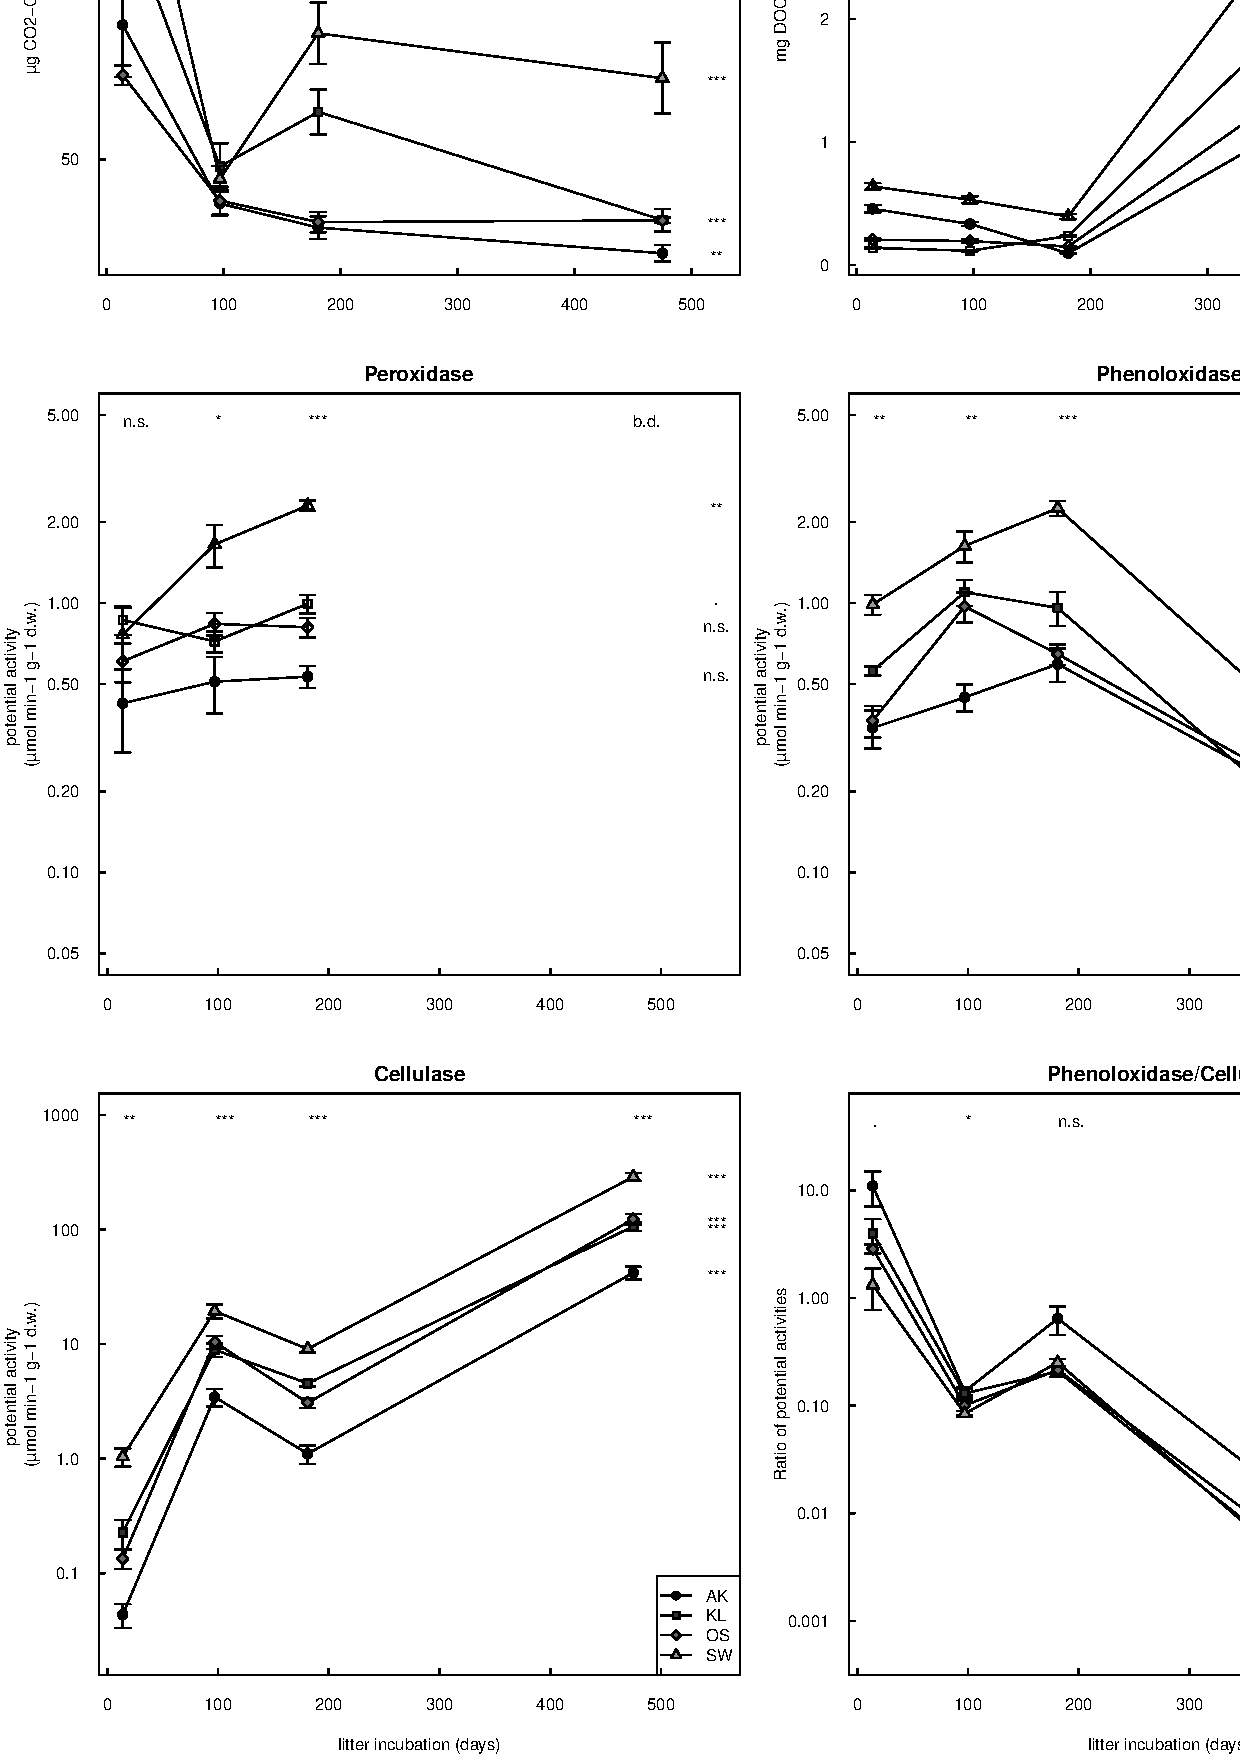
\includegraphics{ligpaper-enz}
\end{center}
\caption{
{\bf Respiration rates, concentration of soluble organic C and potential extracellular enzyme activities} in decomposing beech leaf litter from a mesocosm experiment. Beech litter was collected in: triangles, Schottenwald (SW); diamonds, Ossiach (OS); squares, Klaus-nleopoldsdorf (KL); circles, Achenkirch, AK. Error bars indicate standard errors (n=5). Significant differences between litter types are presented by asterisks above the symbols, significant differences between time points by asterisks to the right of the curves. *, P\textless 0.05, **, P\textless 0.01, ***, P\textless 0.001, b.d. - below detection limit.}
\label{fig:enz}
\end{figure}

\begin{figure}[!ht]
\begin{center}
%\setkeys{Gin}{width=4in}
\setkeys{Gin}{width=\textwidth}
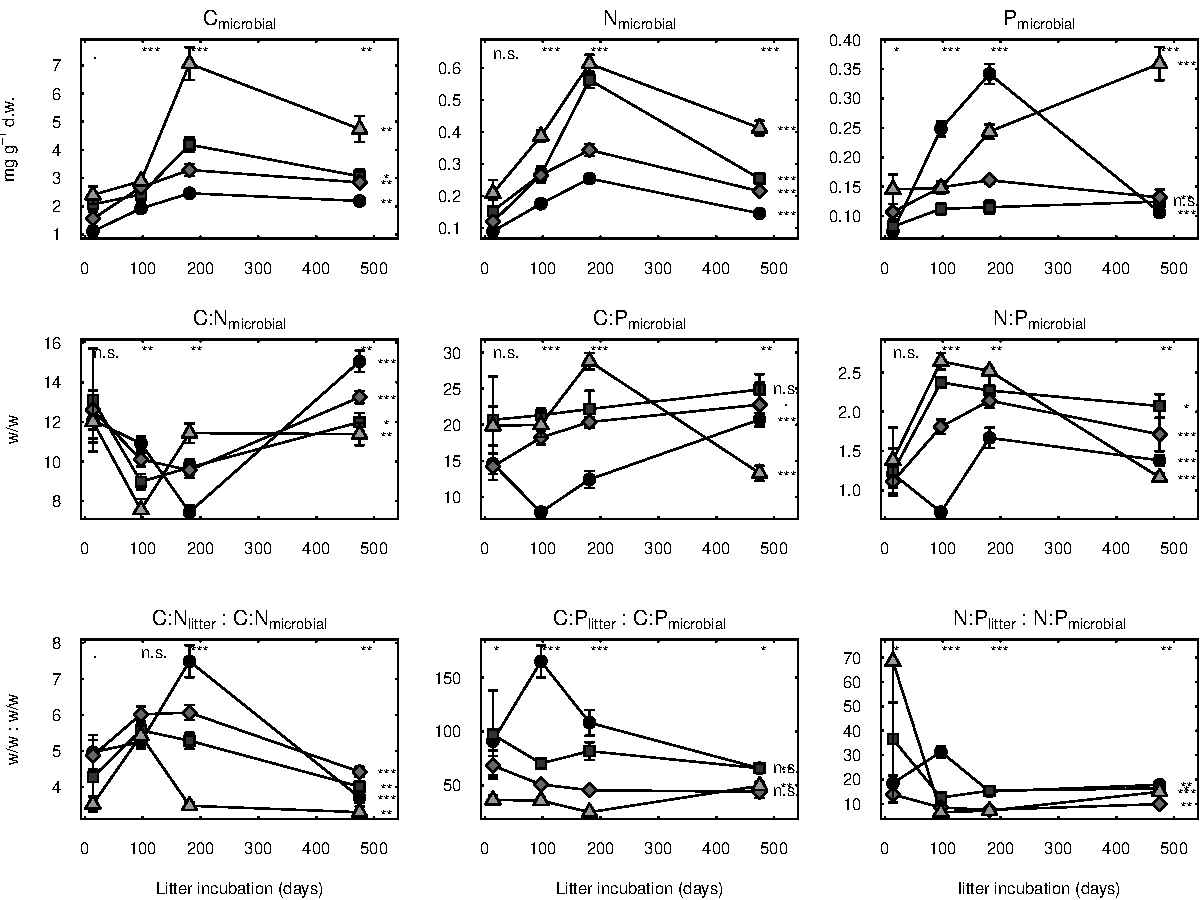
\includegraphics{ligpaper-mb}
\end{center}
\caption{
{\bf Microbial biomass C, N and P, microbial C:N:P stoichiometry and resource/consumer stoichiometric imbalance in these elements}in decomposing beech leaf litter from a mesocosm experiment. Beech litter was collected in: triangles, Schottenwald (SW); diamonds, Ossiach (OS); squares, Klausenleopoldsdorf (KL); circles, Achenkirch, AK. Error bars indicate standard errors (n=5). Significant differences between litter types are presented by asterisks above the symbols, significant differences between time points by asterisks to the right of the curves. *, P\textless 0.05, **, P\textless 0.01, ***, P\textless 0.001.}
\label{fig:mb}
\end{figure}

\newpage
\begin{figure*}[h!]
\vspace*{2mm}
\begin{center}
\setkeys{Gin}{width=\textwidth}
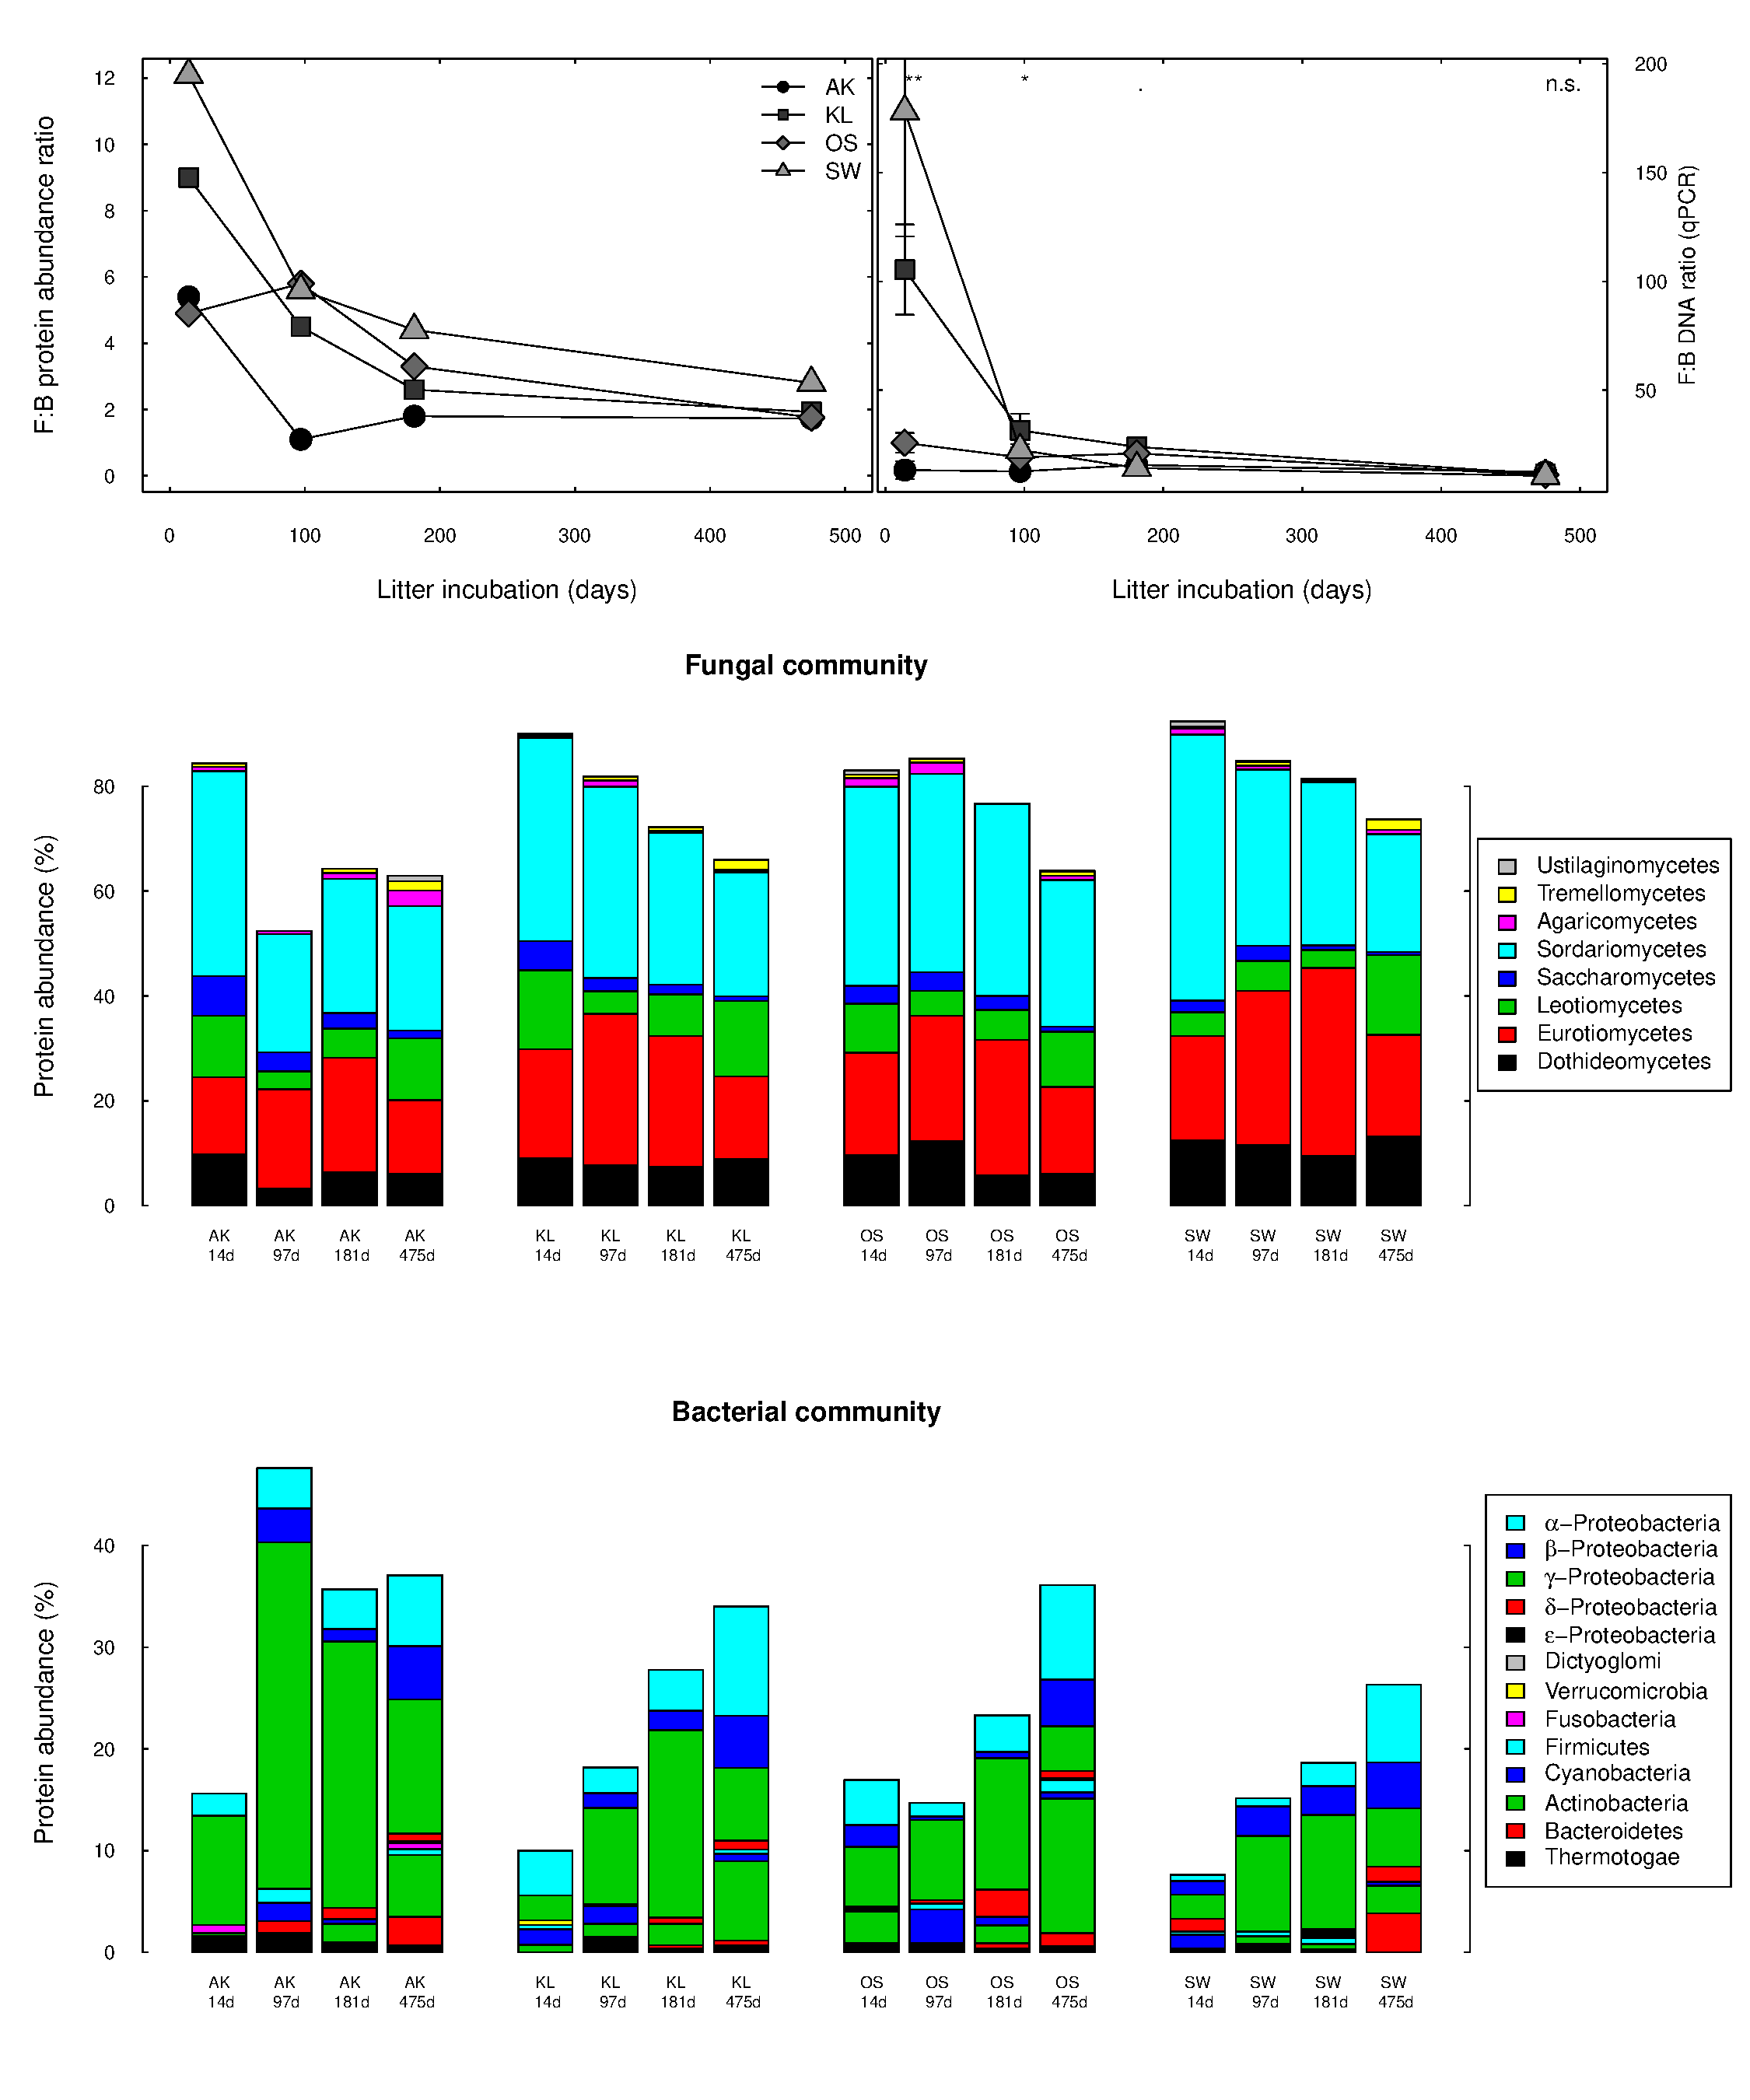
\includegraphics{ligpaper-metaprot2}
\end{center}
\caption{
{\bf Protein abundance of fungal and bacterial taxa.}}
\label{fig:metaprot_barplot}
\end{figure*}


\begin{figure}[!ht]
\begin{center}
\setkeys{Gin}{width=0.7\textwidth}
%\inputgraphics[width=4in]{figure_name.2.eps}
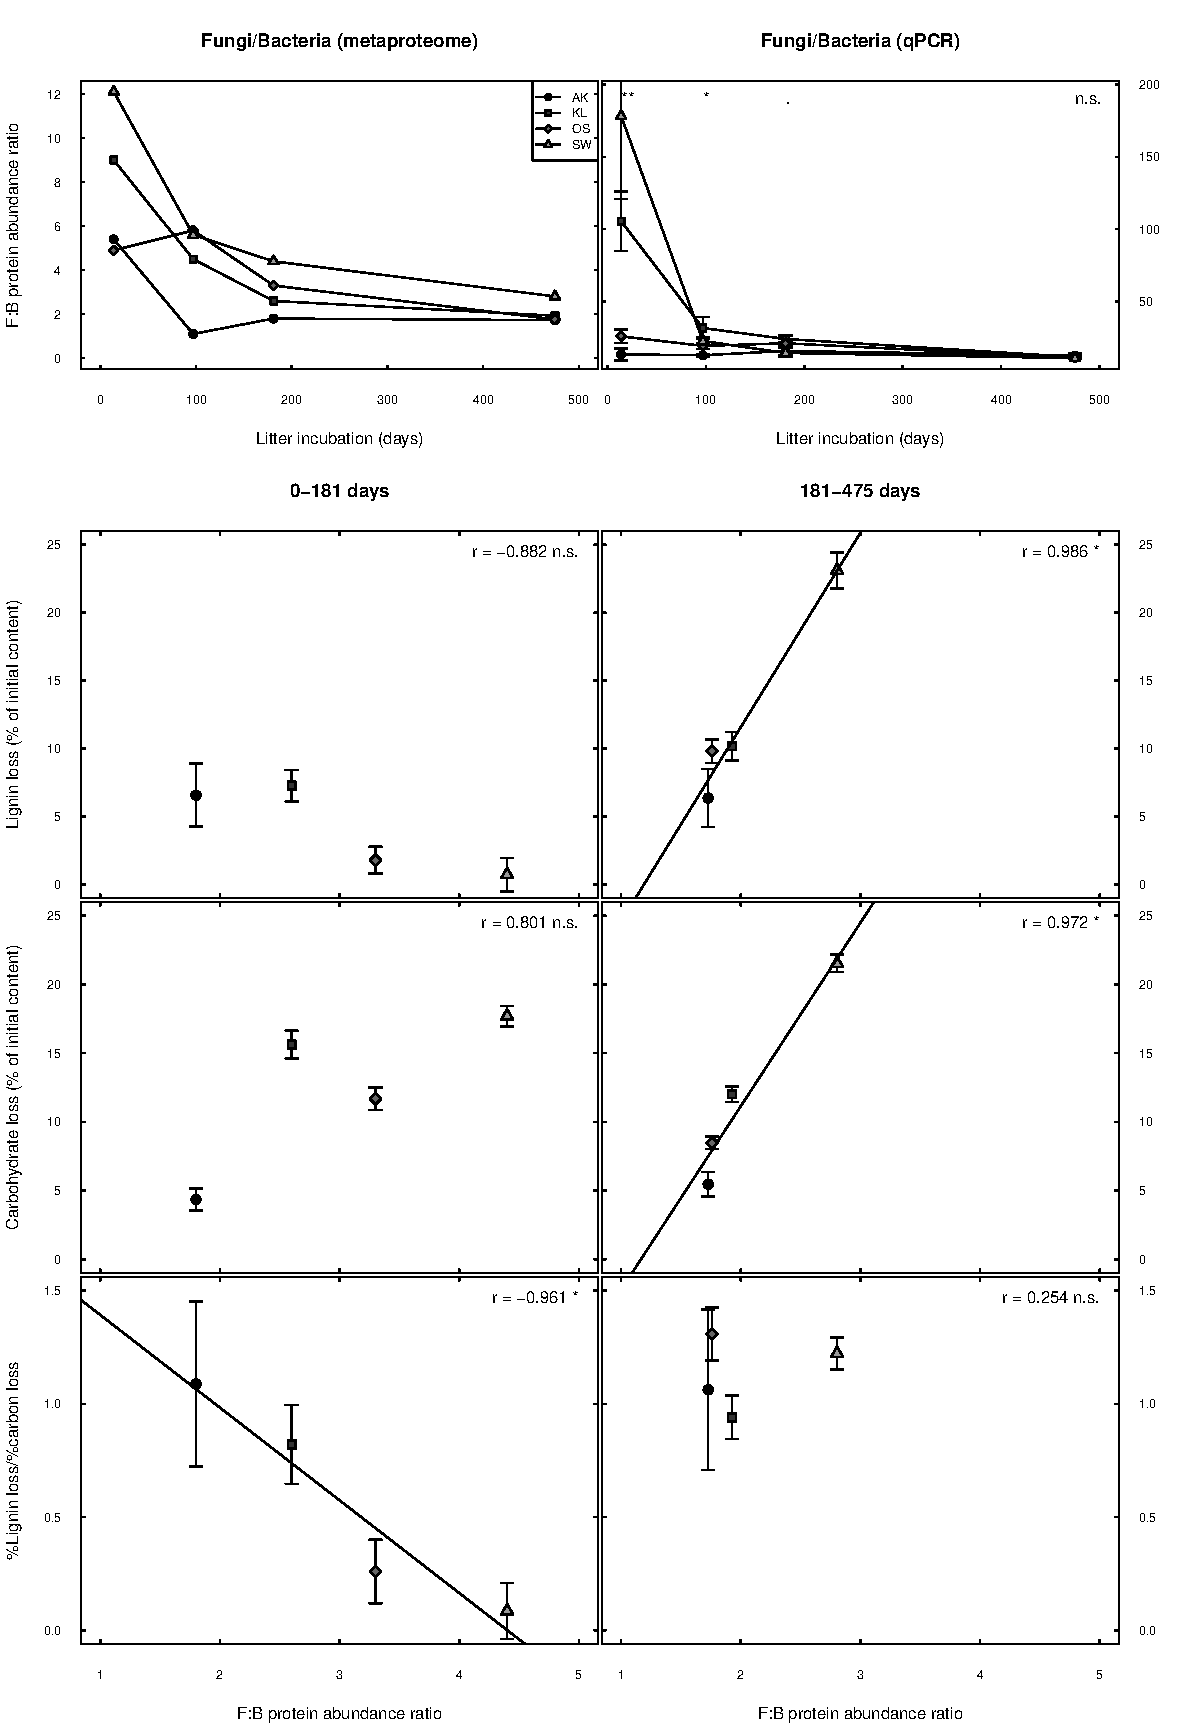
\includegraphics{ligpaper-f2bnew}
\end{center}
\caption{
{\bf Fungi:Bacteria (F:B) ratios and their correlations with LCI change:} Top: F:B protein abundance (left) and DNA (right) ratio. Bottom: Correlations between F:B preotein abundance ratios and Lignin loss (mid) and lignin loss / carbon loss (bottom) for 0-6 months (left) and 6-15 months (right..Errorbars indicate standard errors (n=4-5).  Beech litter was collected in: triangles, Schottenwald (SW); diamonds, Ossiach (OS); squares, Klausenleopoldsdorf (KL); circles, Achenkirch, AK. Error bars indicate standard errors (n=5). Significant differences between litter types are presented by asterisks above the symbols, significant differences between time points by asterisks to the right of the curves. *, P\textless 0.05, **, P\textless 0.01, ***, P\textless 0.001.}
\label{fig:f2b}
\end{figure}

\newpage
\begin{figure}[!ht]
\begin{center}
%\setkeys{Gin}{width=4in}
\setkeys{Gin}{width=\textwidth}
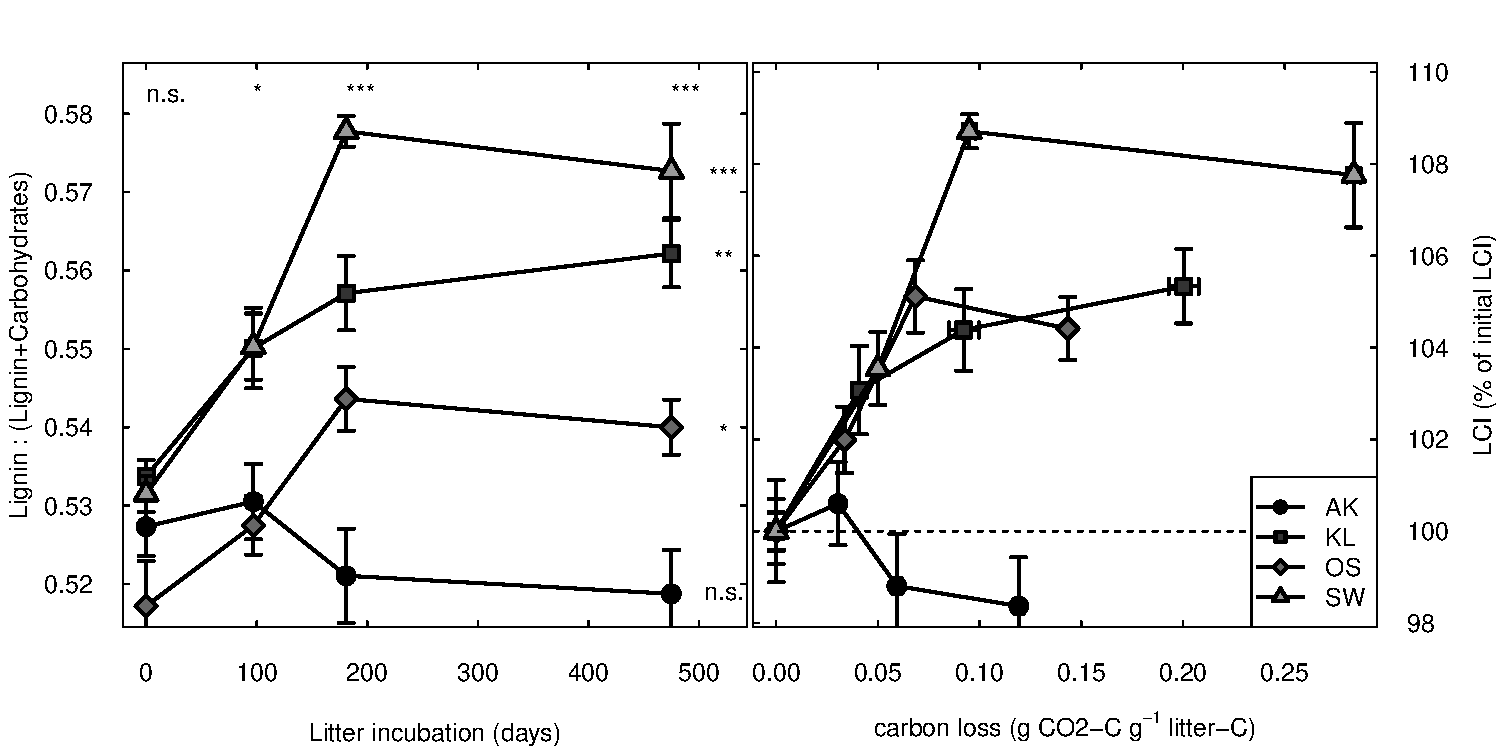
\includegraphics{ligpaper-lci}
\end{center}
\caption{
{\bf Develoment of the LCI (lignin/(lignin+carbohydrates))} during time of beech litter decomposition (A) or plotted against cumulative C loss (B). Errorbars indicate standard errors (n=4-5). The dashed line indicates a constant ratio between lignin and carbohydrates (i.e. no preferential decomposition of carbohydrates. Beech litter was collected in: triangles, Schottenwald (SW); diamonds, Ossiach (OS); squares, Klausenleopoldsdorf (KL); circles, Achenkirch, AK. Error bars indicate standard errors (n=5). Significant differences between litter types are presented by asterisks above the symbols, significant differences between time points by asterisks to the right of the curves. *, P\textless 0.05, **, P\textless 0.01, ***, P\textless 0.001.}
\label{fig:lci}
\end{figure}


\newpage
\begin{figure*}[h!]
\vspace*{2mm}
\begin{center}
\setkeys{Gin}{width=\textwidth}
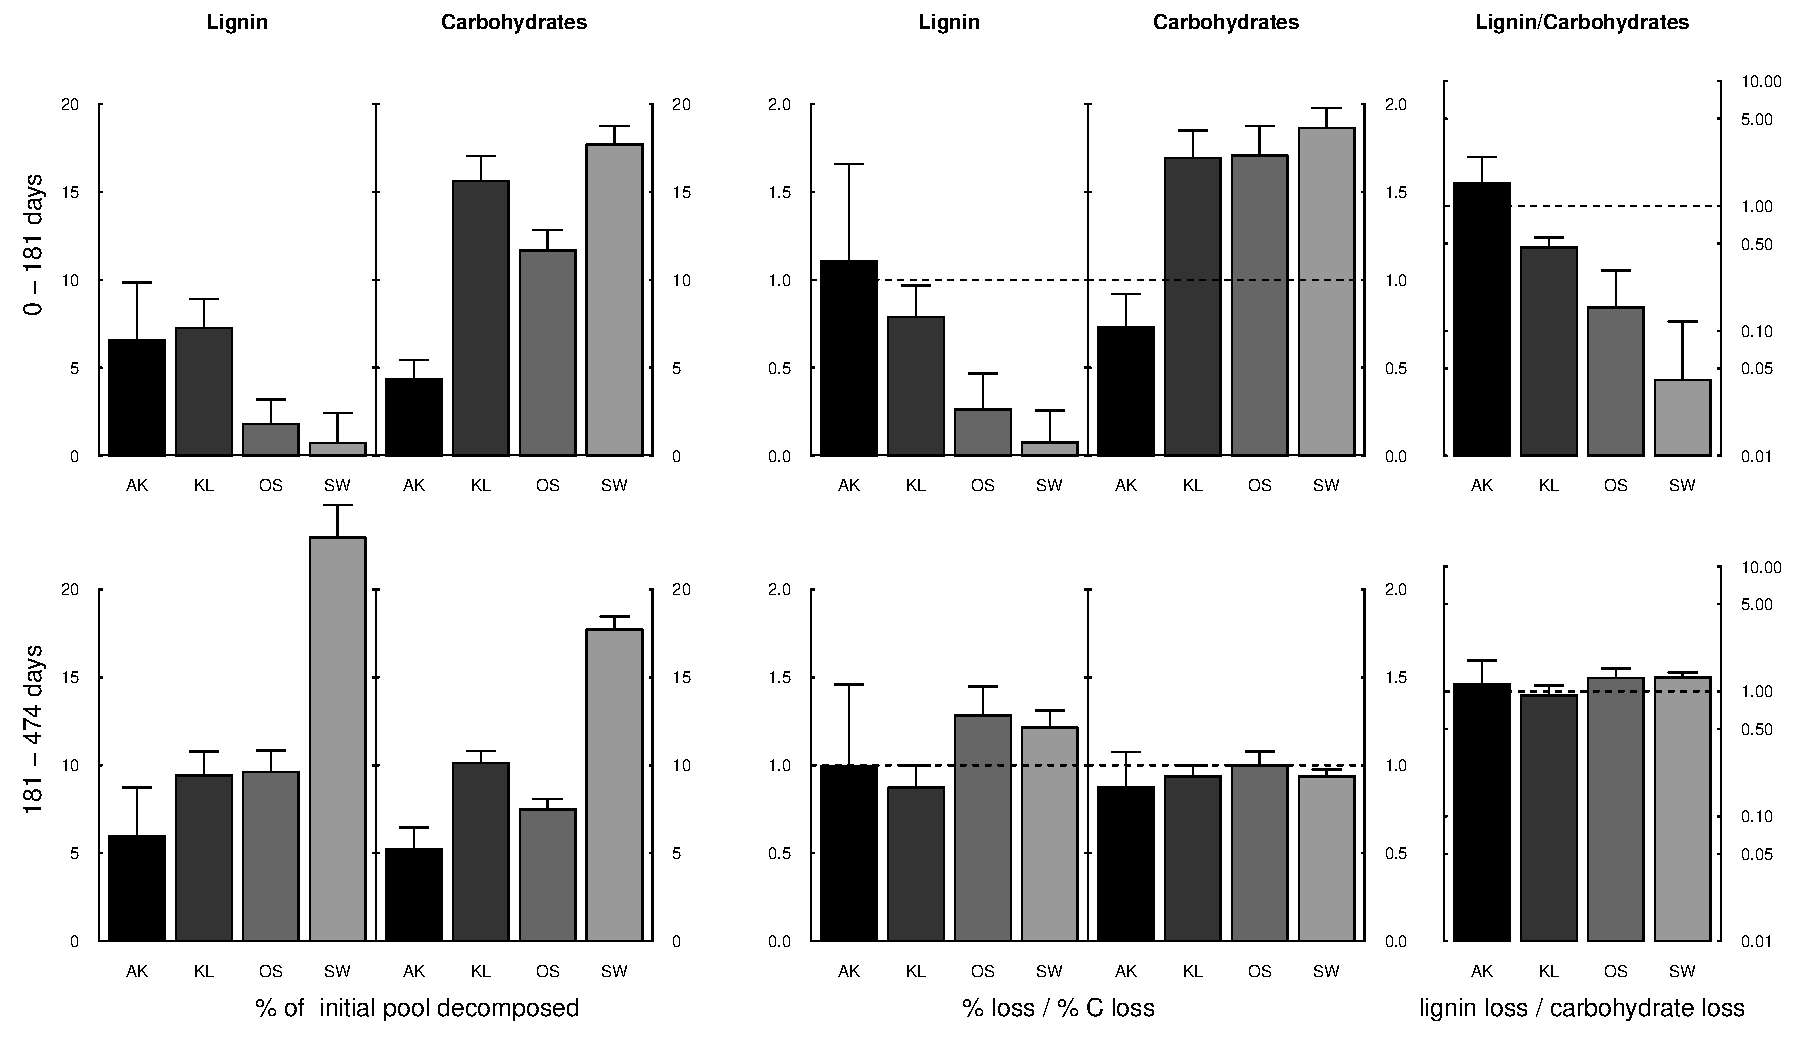
\includegraphics{ligpaper-degrdiff}
\end{center}
\caption{
{\bf Carbon loss corrected amounts of lignin and carbohydrates} degraded in beech litter collected in Achenkirch (AK), Klausenleopoldsdorf (KL), Ossiach (OS) and Schottenwald (SW). Carbon loss was calculated based on accumulated respiration for each mesocosm. Error bars indicate standard errors (n=4-5). The dashed line marks no discrimation during decomposition between lignin, carbohydrates and bulk carbon}
\label{fig:degr}
\end{figure*}

\newpage
\begin{figure*}[h!]
\vspace*{2mm}
\begin{center}
\setkeys{Gin}{width=\textwidth}
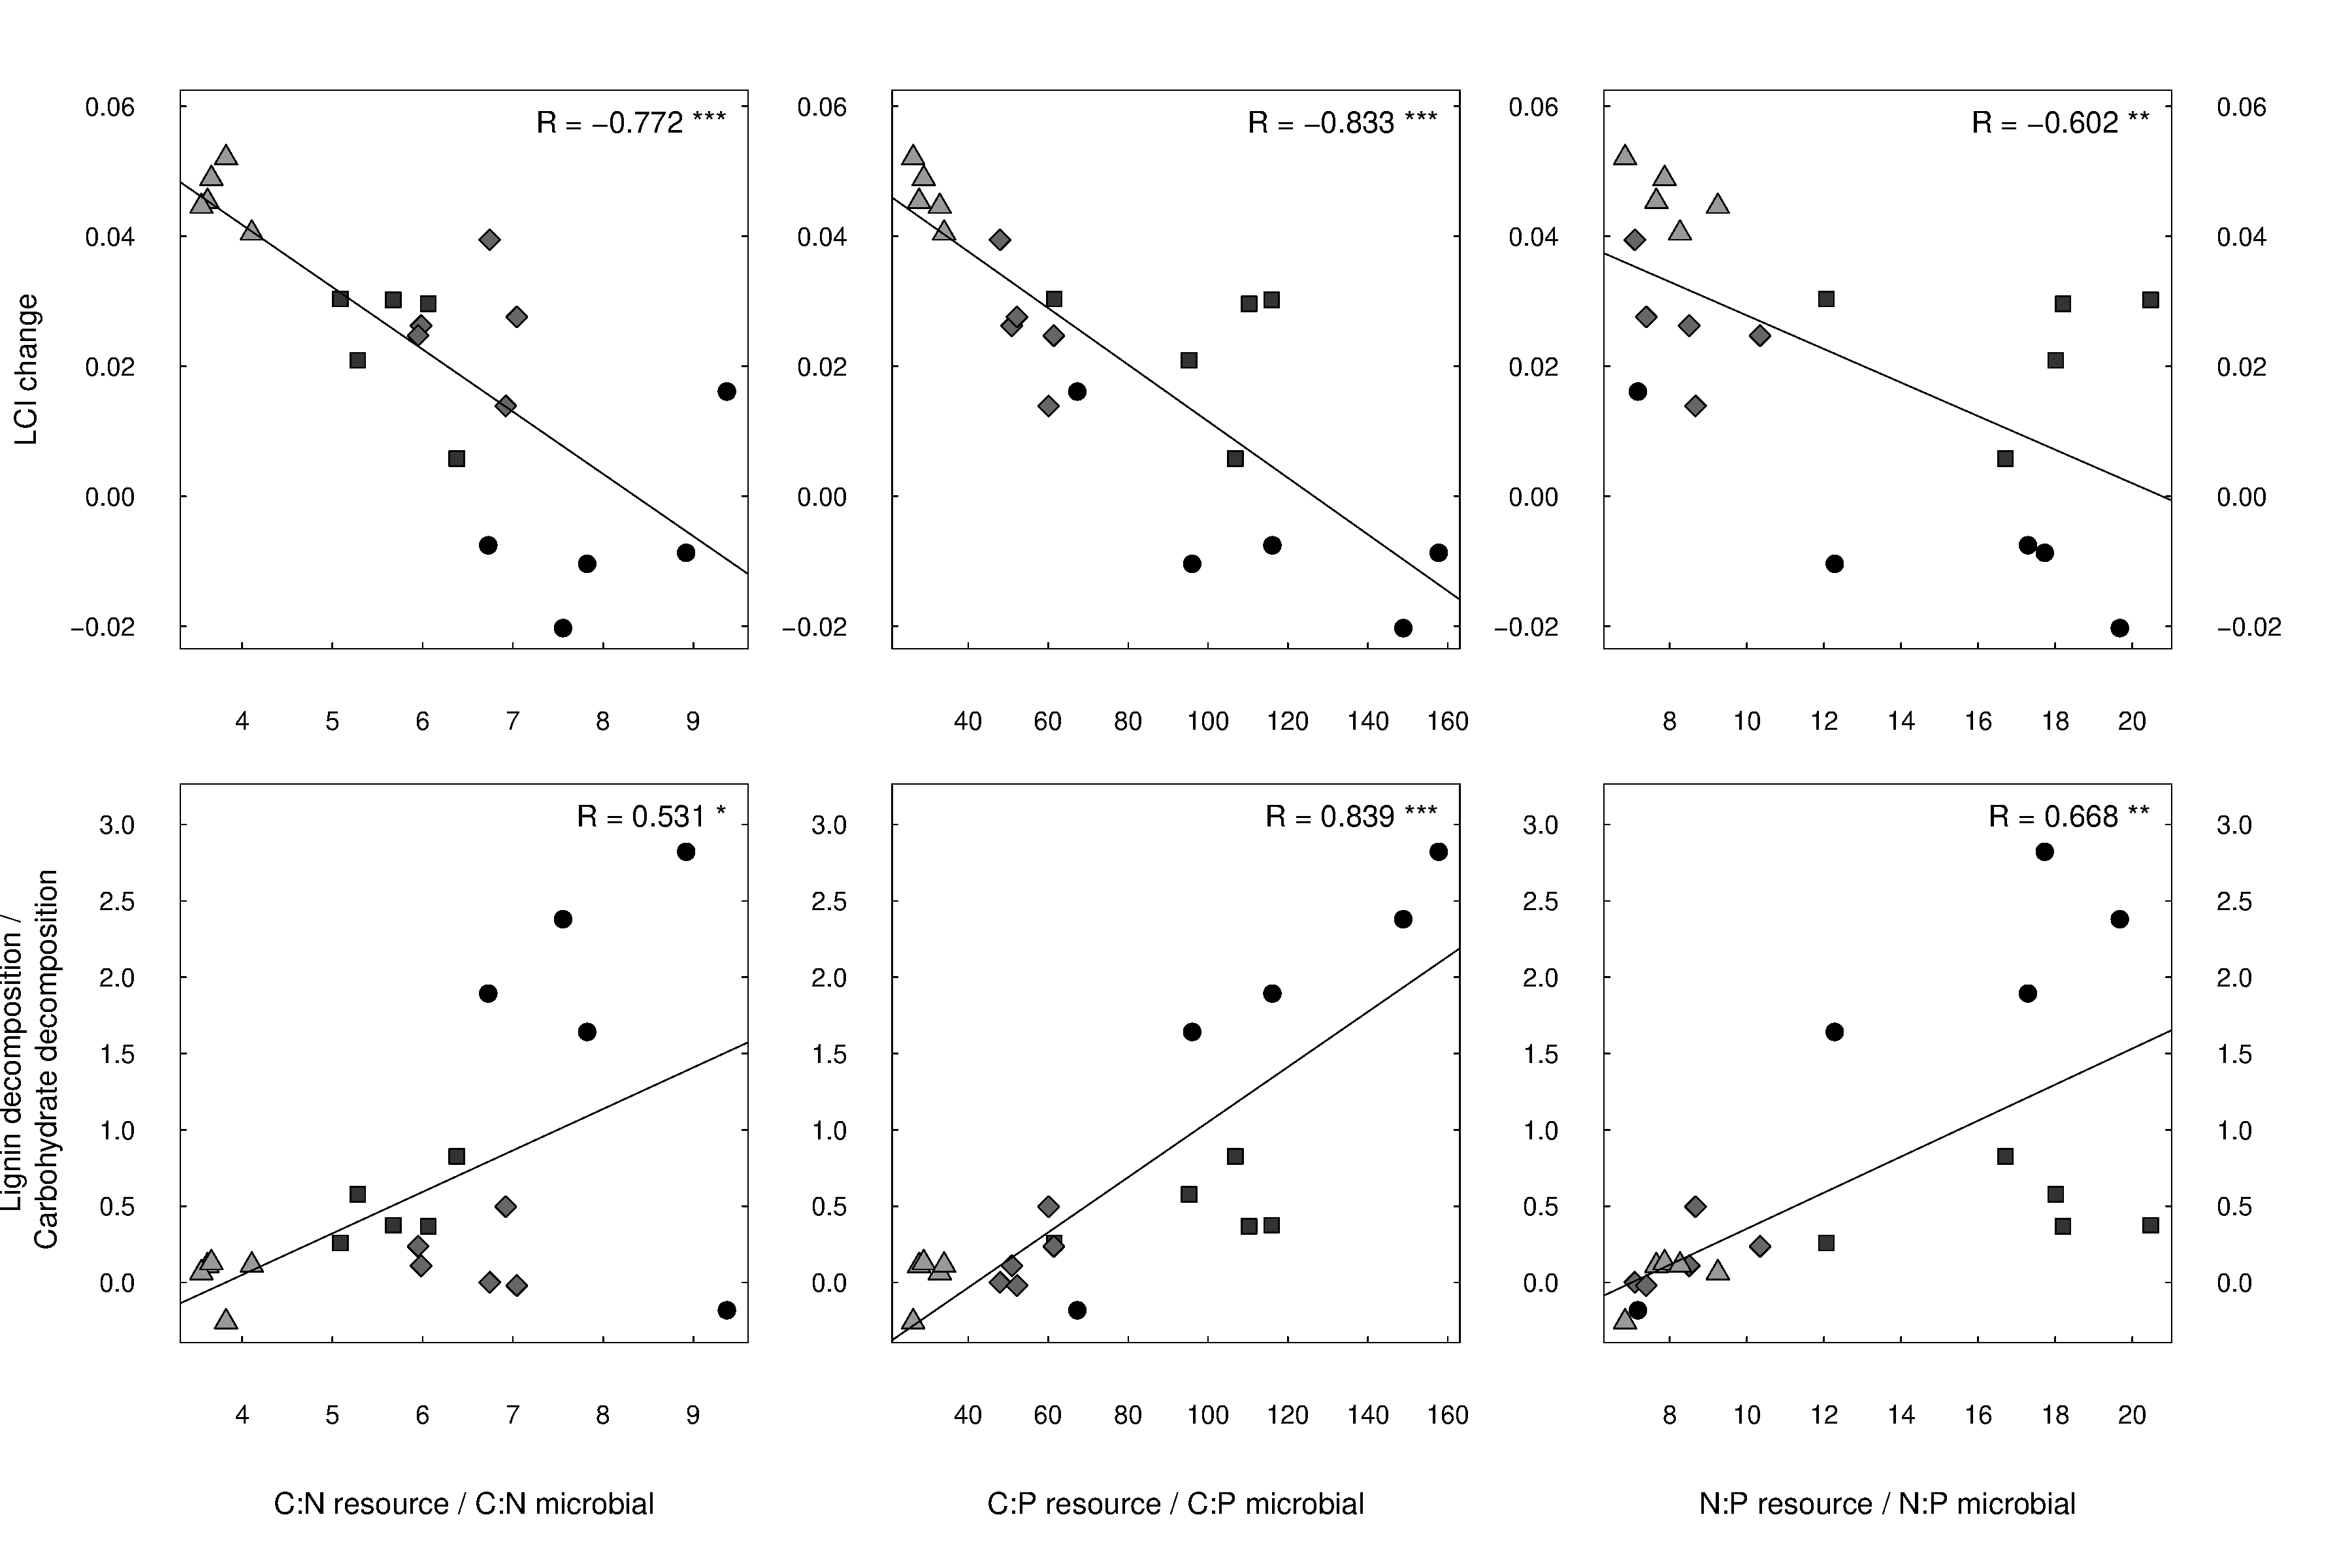
\includegraphics{ligpaper-graphcorr}
\end{center}
\caption{
{\bf Correlation between the LCI change or the ratio of lignin/carbohydrate decomposition ratio during the first 6 months of litter decomposition correlate to litter/microbe stoichiometric imbalances.} and change and Correlations between lignin accumulation during the first 6 month of litter incubation and stoichiometric resource:consumer imbalances. LCI is calculates as of lignin/(lignin+Carbohydrates).  Beech litter was collected in: triangles, Schottenwald (SW); diamonds, Ossiach (OS); squares, Klausenleopoldsdorf (KL); circles, Achenkirch, AK. *, P\textless 0.05, **, P\textless 0.01, ***, P\textless 0.001.}
\label{fig:cor1}
\end{figure*}



\newpage
\begin{figure*}[h!]
\vspace*{2mm}
\begin{center}
\setkeys{Gin}{width=\textwidth}
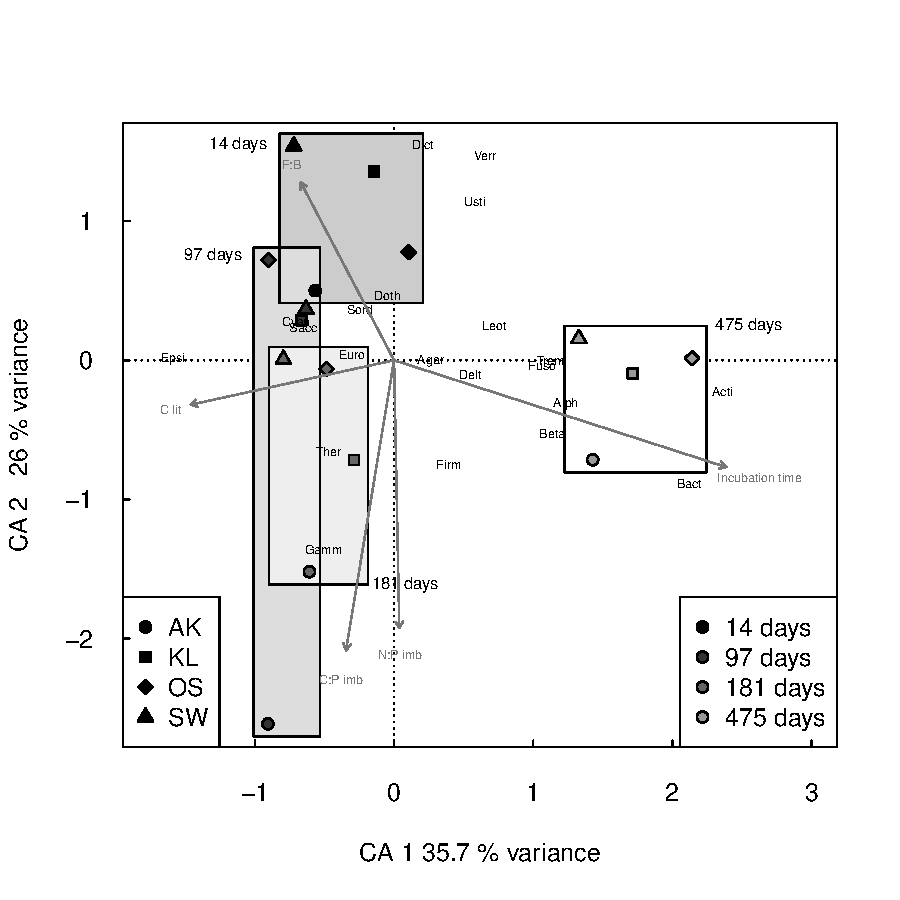
\includegraphics{ligpaper-metaprot_pca}
\end{center}
\caption{
{\bf Microbial commuity composition.} The first two components of a correspondance analysis (CA) of protein abundances found. Rectangles indicate samples of identical incubation time. Peptides were aggregated at class level (fungi and proteobacteria) or phylum level (other bacterial phyla): Dothideomycetes (Doth); Eurotiomycetes (Euro); Leotiomycetes (Leot); Saccharomycetes (Sacc); Sordariomycetes (Sord); Agaricomycetes (Agar); Tremellomycetes (Trem); Ustilaginomycetes (Usti); Thermotogae (Ther); Bacteroidetes (Bact); Actinobacteria (Acti); Cyanobacteria (Cyan); Firmicutes (Firm); Fusobacteria (Fuso); Verrucomicrobia (Verr); Dictyoglomi (Dict); Alphaproteobacteria (Alph); Betaproteobacteria (Beta); Gammaproteobacteria (Gamm); Deltaproteobacteria (Delt); Epsilonproteobacteria (Epsi). Taxa factor loadings were printed x2 for better readability. Correlations between CA 1, CA 2, and litter chemistry, microbial stoichiometry, and protein abundance of microbial taxa are stated in supplemental table \ref{catab}. Arrows represent vectorial fittings of these variables calculated independently from the CA, plotted only if p\textless 0.05: Litter C content (C lit); C:X\textsubscript{Microbial}/C:X\textsubscript{Litter} (C:P imb, C:N imb).}
\label{fig:metaprotpca}
\end{figure*}

\newpage


\section*{Supporting Information}

\newpage
\begin{landscape}
% latex table generated in R 2.12.1 by xtable 1.5-6 package
% Sat Nov  5 23:56:54 2011
\begin{table}[h!]
%\begin{center}
\caption{Element concentrations, elemental stoichiometry and cellulose and lignin concentrations in beech litter measured after 14 days incubation. Standard errors are given in brackets (n=5). C extr represents for soluble organic carbon. Beech litter was collected in AK, Achenkirch, KL, Klausenleopoldsdorf, OS, Ossiach, and SW, Schottenwald.}
\label{initstoech}

{\small
\begin{tabular}{lrlrlrlrlrlr}
  \hline
 & AK & (SE) & KL & (SE) & OS & (SE) & SW & (SE) & p value \\ 
  \hline
C (\% d.w.) & 50.86 & (0.39) & 49.41 & (0.53) & 48.15 & (0.39) & 48.90 & (0.34) & 0.002 \\ 
  C extr (mg g-1) & 0.46 & (0.03) & 0.14 & (0.01) & 0.21 & (0.01) & 0.64 & (0.03) & $<$0.001 \\ 
  N (\% d.w.) & 0.878 &  (0.012) & 0.938 &  (0.012) & 0.806 &  (0.013) & 1.172 &  (0.016) & $<$0.001 \\ 
  P (\% d.w.) & 0.040 & (0.000) & 0.030 & (0.000) & 0.052 & (0.002) & 0.070 & (0.000) & $<$0.001 \\ 
  C:N (w/w) & 57.86 &  (0.57) & 52.60 &  (0.49) & 59.97 &  (0.72) & 41.78 &  (0.76) & $<$0.001 \\ 
  C:P (w/w) & 1282 & (21) & 1548 & (25) & 905 & (15) & 699 & (9) & $<$0.001 \\ 
  N:P (w/w) & 22.17 & (0.47) & 29.45 & (0.60) & 15.10 & (0.29) & 16.75 & (0.39) & $<$0.001 \\ 
  K (mg g-1) & 0.26 & (0.00) & 0.54 & (0.00) & 0.21 & (0.00) & 0.55 & (0.00) & $<$0.001 \\ 
  Ca (mg g-1) & 1.33 & (0.01) & 1.26 & (0.01) & 1.63 & (0.01) & 1.23 & (0.01) & $<$0.001 \\ 
  Mg (mg g-1) & 0.27 &  (0.00) & 0.14 &  (0.00) & 0.20 &  (0.00) & 0.15 &  (0.00) & $<$0.001 \\ 
  Fe (ppm) & 210 & (2) & 208 & (4) & 453 & (12) & 192 & (4) & $<$0.001 \\ 
  Mn (ppm) & 172 &  (2) & 1430 &  (10) & 776 &  (9) & 2137 &  (51) & $<$0.001 \\ 
  Zn (ppm) & 30.8 & (0.4) & 33.0 & (0.3) & 36.0 & (1.0) & 42.4 & (0.7) & $<$0.001 \\ 
  Lignin & 28.9 & (28.9) & 29.9 & (29.9) & 31.2 & (31.2) & 30.5 & (30.5) & $<$0.001 \\ 
  Carbohydrates & 25.9 & (25.9) & 26.1 & (26.1) & 29.2 & (29.2) & 26.9 & (26.9) & $<$0.001 \\ 
   \hline
\end{tabular}
}
%\end{center}
\end{table}
\end{landscape}


\begin{table}[h!]
\begin{center}
\caption{Lignin derrived and other phenolic pyrolysis products}
\label{tab:phprod}

{\small
\begin{tabular}{lcccccc}
  \hline
Name & RT & MW & integrated framents & Origin & Class \\ 
  \hline
Guaiacol & 18.87 & 124 & 109+124 &Lignin&Guaiacyl\\ 
Methylguaiacol & 20.32 & 138 & 123+138 &Lignin&Guaiacyl\\ 
Ethylguaiacol & 21.40 & 152 & 137+152 &Lignin&Guaiacyl\\ 
Propenylguaiacol & 23.29 & 164 & 149+164 &Lignin&Guaiacyl\\ 
Vinylguaiacol & 23.69 & 150 & 135+150 &Lignin&Guaiacyl\\ 
Propenylguaiacol & 24.48 & 164 & 149+164 &Lignin&Guaiacyl\\ 
Syringol & 24.58 & 154 & 139+154 &Lignin&Syringyl\\ 
Propenylguaiacol & 25.66 & 164 & 149+164 &Lignin&Guaiacyl\\ 
Methylsyringol & 25.67 & 168 & 153+168 &Lignin&Syringyl\\ 
Ethylsysringol & 26.39 & 182 & 167+182 &Lignin&Syringyl\\ 
Propenylsyringol & 27.97 & 194 & 179+194 &Lignin&Syringyl\\ 
Vinylsyringol & 28.37 & 180 & 165+180 &Lignin&Syringyl\\ 
Guaiacolaldehyde & 28.40 & 152 & 109+152 &Lignin&Guaiacyl\\ 
Propylguaiacol & 28.72 & 166 & 137+166 &Lignin&Guaiacyl\\ 
Oxo-hydroxy-etylguaiacol & 28.77 & 182 & 182 &Lignin&Guaiacyl\\ 
Propenylsyringol & 28.91 & 194 & 179+194 &Lignin&Syringyl\\ 
Oxo-ethylguaiacol & 29.20 & 166 & 151+166 &Lignin&Guaiacyl\\ 
Oxo-propylguaiacol & 29.36 & 180 & 137+180 &Lignin&Guaiacyl\\ 
Propenylsyringol & 30.16 & 194 & 194+179 &Lignin&Syringyl\\ 
Syringolaldehyde & 32.68 & 182 & 139+182 &Lignin&Syringyl\\ 
Oxo-hydroxy-ethylsyringol & 32.80 & 212 & 212 &Lignin&Syringyl\\ 
Guaiacolacetic acid & 32.88 & 182 & 137+182 &Lignin&Guaiacyl\\ 
Propylsyringol & 33.15 & 196 & 181+196 &Lignin&Syringyl\\ 
Oxo-propylsyringol & 33.32 & 210 & 167+210 &Lignin&Syringyl\\ 
Oxopropenylguaiacol & 35.30 & 178 & 135+178 &Lignin&Guaiacyl\\ 
Hydroxypropenylguaiacol & 37.10 & 180 & 137+180 &Lignin&Guaiacyl\\ 
Syringolacetic acid & 38.78 & 212 & 212 &Lignin&Syringyl\\ 
Oxo-propenylsyringol & 43.06 & 208 & 165+208 &Lignin&Syringyl\\ 
Phenol & 21.02 & 94 & 65+66+94 &Phenolic&\\ 
4-Methylphenol & 22.11 & 108 & 107+108 &Phenolic&\\ 
3-Methylphenol & 22.22 & 108 & 107+108 &Phenolic&\\ 
Ethylphenol & 23.38 & 122 & 107+122 &Phenolic&\\ 
Propenylphenol & 26.93 & 134 & 133+134 &Phenolic&\\ 
Propenylphenol & 27.76 & 134 & 133+134 &Phenolic&\\ 
Propylphenol & 31.11 & 136 & 151+166 &Phenolic&\\ 
Butylphenol & 31.86 & 150 & 107+150 &Phenolic&\\ 
4-Hydroxybenzaldehyde & 32.70 & 122 & 121+122 &Phenolic&\\ 
Hydroquinone & 33.40 & 110 & 81+110 &Phenolic&\\ 
   \hline
\end{tabular}
}
\end{center}
\end{table}
\newpage

% latex table generated in R 2.12.1 by xtable 1.6-0 package
% Tue Nov  8 06:46:38 2011
\begin{table}[h!]
\begin{center}
\caption{Carbohydrate derrived pyrolysis products}
\label{tab:chprod}
{\small
\begin{tabular}{lcccccc}
  \hline
Name & RT & MW & integrated framents & Origin & Class \\ 
  \hline
Acetaldehyde & 2.06 & 44 & 29+44 &Carbohydrates&  \\ 
Furan & 2.35 & 68 & 39+68 &Carbohydrates&Furan\\ 
Methylfuran & 2.74 & 82 & 81+82 &Carbohydrates&Furan\\ 
Methylfuran & 2.91 & 82 & 81+82 &Carbohydrates&Furan\\ 
Dimethylfuran & 3.43 & 96 & 95+96 &Carbohydrates&Furan\\ 
Dimethylfuran & 3.66 & 96 & 95+96 &Carbohydrates&Furan\\ 
Vinylfuran & 5.01 & 94 & 65+94 &Carbohydrates&Furan\\ 
Unknown furan & 6.36 & 108 & 107+108 &Carbohydrates&Furan\\ 
Cyclopentanone & 6.99 & 105? & 84+105? &Carbohydrates&Cyclopentenone\\ 
Methylfuran & 7.62 & 82 & 53+82+83 &Carbohydrates&Furan\\ 
2-Oxopropanoic acid, methylester & 7.92 & 102 & 43+102 &Carbohydrates& \\ 
1-Hydroxypropanone & 9.24 & 74 & 43 &Carbohydrates& \\ 
2-Cyclopenten-1-one & 10.26 & 82 & 53+54+52 &Carbohydrates&Cyclopentenone\\ 
2-Methyl-2-cyclopenten-1-one & 10.51 & 96 & 53+96 &Carbohydrates&Cyclopentenone\\ 
1-Hydroxy-2-propanone & 10.69 & 88 & 57+88 &Carbohydrates&Cyclopentenone\\ 
Unknown & 11.38 & unk & 65+66+94 &Carbohydrates& \\ 
3-Furaldehyd & 11.57 & 96 & 95+96 &Carbohydrates&Furan\\ 
2(5H)Furanon & 11.69 & 98 & 55+98 &Carbohydrates&Furan\\ 
Propanoic acid, methylester & 12.10 & 102 & 43+102 &Carbohydrates& \\ 
2-Furaldehyd & 12.22 & 96 & 95+96 &Carbohydrates&Furan\\ 
Acetylfuran & 12.99 & 110 & 95+110 &Carbohydrates&Cyclopentenone\\ 
3-Methyl-cyclopentanone & 13.31 & 96 & 67+96 &Carbohydrates&Cyclopentenone\\ 
Dimethylcyclopentenone & 13.69 & 110 & 67+95+110 &Carbohydrates&Cyclopentenone\\ 
5-Methyl-2-furancarboxaldehyde & 14.23 & 110 & 109+110 &Carbohydrates&Furan\\ 
2-Cyclopenten-1,4-dione & 14.44 & 96 & 54+68+96 &Carbohydrates&Cyclopentenone\\ 
Butyrolactone & 15.22 & 86 & 56+86 &Carbohydrates& \\ 
Unknown & 15.56 &  &  &Carbohydrates&  \\ 
Furanmethanol & 15.61 & 98 & 98 &Carbohydrates&Cyclopentenone\\ 
5-Methyl-2(5H)-furanone & 16.06 & 98 & 55+98 &Carbohydrates&Furan\\ 
Unknown & 16.17 & unk & 110 &Carbohydrates&  \\ 
1,2-Cylopentandione & 17.51 & 98 & 55+98 &Carbohydrates&Cyclopentenone\\ 
Unknown & 17.67 & unk & 42+70 &Carbohydrates&  \\ 
2-Hydroxy-3-methyl-2-cyclopenten-1-one & 18.14 & 98 & 98 &Carbohydrates&Cyclopentenone\\ 
3-Methy-l1,2-cyclopentanedione & 18.42 & 112 & 69+112 &Carbohydrates&Cyclopentenone\\ 
Unknown & 19.06 && 58+86+114 &Carbohydrates&\\ 
Unknown & 19.35 && 98+126 &Carbohydrates&\\ 
Unknown & 21.77 && 116 &Carbohydrates&\\ 
Unknown & 22.33 && 44 &Carbohydrates&\\ 
Unknown & 26.18 && 57+69 &Carbohydrates&\\ 
5-Hydroxymethylfuran-1-carboxaldehyde & 27.51 & 126 & 97+126 &Carbohydrates&Furan\\ 
Unknown & 31.67 && 73+135 &Carbohydrates&\\ 
Laevoglucosan & 40.44 & 172 & 60+73 &Carbohydrates& \\ 
   \hline
\end{tabular}
}
\end{center}
\end{table}


\newpage
% latex table generated in R 2.12.1 by xtable 1.6-0 package
% Tue Nov  8 06:46:38 2011
\begin{table}[h!]
\begin{center}
\caption{Other pyrolysis products quantified}
\label{tab:nprod}
{\small
\begin{tabular}{lcccccc}
  \hline
Name & RT & MW & integrated framents & Origin & Class \\ 
  \hline
25:0 Alkan & 27.74 & 352 & 57+71 &aliphatic& Alkan \\ 
25:1 Alken & 28.34 & 350 & 57+69 &aliphatic& Alken \\ 
27:0 Alkan & 30.04 & 380 & 57+67 &aliphatic& Alkan \\ 
27:1 Alken & 30.63 & 378 & 57+65 &aliphatic& Alken \\ 
29:0 Alkan & 32.20 & 408 & 57+63 &aliphatic& Alkan \\ 
29:1 Alken & 32.82 & 406 & 57+61 &aliphatic& Alken \\ 
Myristic acid (14:0) & 2.35 & 68 & 39+68 & Lipid & Fatty Acid \\ 
Palmitic acid (16:0) & 2.74 & 82 & 81+82 & Lipid & Fatty Acid \\ 
Stearuc acid (18:0) & 2.91 & 82 & 81+82 & Lipid & Fatty Acid \\ 
N-methyl-pyrrol & 6.15 & 81 & 80+81 &Protein& Pyrrol \\ 
Pyridine & 6.90 & 95 & 52+79+95 &Protein& Pyridine \\ 
Methylpyridine & 7.50 & 93 & 66+92+93 &Protein& Pyridine \\ 
Methylpyridine & 7.54 & 93 & 66+92+93 &Protein& Pyridine \\ 
methylpyridine & 9.02 & 93 & 66+93 &Protein& Pyridine \\ 
Pyrrol & 13.11 & 67 & 39+41+67 &Protein& Pyrrol \\ 
Methylpyrrol & 13.81 & 81 & 80+81 &Protein& Pyrrol \\ 
Methylpyrrol & 14.10 & 81 & 80+81 &Protein& Pyrrol \\ 
3-Hydroxypyridine & 26.52 & 95 & 67+95 &Protein& Pyridine \\ 
Indole & 26.85 & 117 & 89+117 &Protein& Indole \\ 
Methylindole & 27.42 & 131 & 130+131 &Protein& Indole \\ 
Toluene & 4.54 & 92 & 91+92 &&Aromatic\\ 
Xylene & 5.94 & 106 & 91+105+106 &&Aromatic\\ 
Xylene & 6.09 & 106 & 91+105+106 &&Aromatic\\ 
Xylene & 6.20 & 106 & 91+105+106 &&Aromatic\\ 
Xylene & 6.99 & 105? & 84+105? &&Aromatic\\ 
Methoxytoluene & 11.78 & 122 & 121+122 &&Aromatic\\ 
Indene & 12.64 & 116 & 115+116 &&Aromatic\\ 
Benzaldehyde & 13.35 & 106 & 77+106 &&Aromatic\\ 
Dihydrobenzofuran & 26.19 & 120 & 91+119+120 &  & Aromatic \\ 
Limonene & 7.22 & 136 & 93 && Terpene \\ 
Phytol & 20.00 & 276 & 95+123 & Chlorophyll & Terpene \\ 
Unknown aliphatic & 22.82 && 58+71 && aliphatic \\ 
Aceton & 2.46 & 58 & 43 &  &  \\ 
2-Propenal & 2.60 & 56 & 55+56 &  &\\ 
Methanol & 2.88 & 32 & 29+31+32 &  &\\ 
3-Buten-2-one & 3.39 & 70 & 55+70 &  &\\ 
2,3-Butandione & 3.67 & 86 & 69+86 &&\\ 
3-Penten-2-one & 3.89 & 86 & 69+86 &&\\ 
2-Butanal & 4.56 & 70 & 69+70 &&\\ 
2,3-Pentadione & 4.77 & 100 & 57+100 &&\\ 
Hexanal & 5.16 & 82 & 56+72+82 &&\\ 
1-Penten-3-one & 11.28 & 84 & 55+84 &&\\ 
Hexan-2,4-dion & 23.92 & 114 & 56+84+114 &&  \\ 
unknown & 15.98 && 119+134 &&\\ 
Unknown & 20.85 && 81 &&\\ 
Unknown & 20.86 && 82+95 &&\\ 
Unknown & 22.43 && 98+128 &&\\ 
Unknown & 27.76 && 138 &&\\ 
   \hline
\end{tabular}
}
\end{center}
\end{table}


\begin{landscape}

% latex table generated in R 2.13.1 by xtable 1.6-0 package
% Wed Feb 15 14:23:40 2012
\begin{table}[h!]
\begin{center}
\caption{Results of correlation analysis (R) between lignin and carbohydrate decomposition and other decomposition processes (mass loss, respiration), extracellular enzyme activities, litter chemistry, and litter and microbial biomass C:N:P stoichiometry. Significant (p\textless 0.05) correlations are presented in bold. Data taken from \cite{Mooshammer2011, Leitner2011}. Changes in litter chemistry (lignin and carbohydrate decomposition) were calculated between 0 and 181 days, other data were measured after 181 days. L acc - lignin accumulation, Ch acc - Carbydrate accumulation, LCI - LCI difference, L dec - lignin decomposition rate, C dec - carbohydrate decomposition,  rate, L resp - lignin loss / carbon loss, C resp - carbohydrate loss / carbon loss, L/C dec - lignin loss / carbohydrate loss, Per/Cell - Potetial peroxidase activity / potential cellulase activity, Phen/Cell - Potetial phenolo activity / potential cellulase activity.}
\label{corrtable}
{\small
\begin{tabular}{lrrrrrrrrrr}
  \hline
 & L acc & Ch acc & LCI diff & L dec & C dec & L resp & C resp & L/C dec & Per/Cell & Phen/Cell \\ 
  \hline
Massloss & 0.291 & -0.15 & 0.245 & -0.328 & 0.106 & -0.201 & 0.125 & -0.081 & 0.048 & 0.053 \\ 
  Actual respiration & 0.333 & \textbf{-0.723} & \textbf{0.606} & -0.082 & \textbf{0.771} & -0.195 & \textbf{0.594} & -0.368 & -0.268 & -0.362 \\ 
  Accumulated Respiration & \textbf{0.494} & \textbf{-0.704} & \textbf{0.688} & -0.132 & \textbf{0.856} & -0.332 & \textbf{0.557} & \textbf{-0.525} & \textbf{-0.506} & \textbf{-0.534} \\ 
  Cellulase activity & \textbf{0.657} & \textbf{-0.76} & \textbf{0.803} & -0.431 & \textbf{0.801} & \textbf{-0.497} & \textbf{0.664} & \textbf{-0.589} & -0.436 & \textbf{-0.539} \\ 
  Protease activity & 0.186 & -0.296 & 0.264 & -0.132 & 0.274 & -0.157 & 0.301 & -0.27 & -0.26 & -0.18 \\ 
  Chitinase activity & 0.409 & \textbf{-0.749} & \textbf{0.663} & -0.17 & \textbf{0.795} & -0.312 & \textbf{0.677} & \textbf{-0.559} & \textbf{-0.49} & \textbf{-0.607} \\ 
  Phosphatase activity & \textbf{0.549} & \textbf{-0.813} & \textbf{0.776} & -0.302 & \textbf{0.851} & -0.407 & \textbf{0.702} & \textbf{-0.556} & -0.418 & \textbf{-0.522} \\ 
  Phenooxidase activity & \textbf{0.632} & \textbf{-0.669} & \textbf{0.737} & -0.415 & \textbf{0.719} & \textbf{-0.449} & \textbf{0.552} & \textbf{-0.484} & -0.305 & -0.356 \\ 
  Peroxidase activity & \textbf{0.599} & \textbf{-0.588} & \textbf{0.677} & -0.412 & \textbf{0.639} & -0.438 & \textbf{0.47} & -0.435 & -0.173 & -0.302 \\ 
  N mineralization & \textbf{0.466} & \textbf{-0.664} & \textbf{0.65} & -0.167 & \textbf{0.739} & -0.299 & \textbf{0.527} & -0.387 & -0.282 & -0.367 \\ 
  Nitrification & \textbf{0.587} & \textbf{-0.707} & \textbf{0.732} & -0.38 & \textbf{0.74} & -0.432 & \textbf{0.621} & \textbf{-0.499} & -0.369 & -0.45 \\ 
  P mineralization & \textbf{0.665} & \textbf{-0.55} & \textbf{0.684} & \textbf{-0.544} & \textbf{0.596} & \textbf{-0.576} & 0.414 & \textbf{-0.478} & -0.212 & -0.255 \\ 
  C litter & \textbf{-0.545} & \textbf{0.506} & \textbf{-0.578} & \textbf{0.604} & -0.368 & \textbf{0.643} & \textbf{-0.618} & \textbf{0.698} & \textbf{0.525} & \textbf{0.581} \\ 
  extractable C & \textbf{0.609} & \textbf{-0.766} & \textbf{0.782} & -0.37 & \textbf{0.814} & \textbf{-0.446} & \textbf{0.658} & \textbf{-0.54} & -0.392 & \textbf{-0.484} \\ 
  N litter & 0.354 & \textbf{-0.517} & \textbf{0.503} & -0.14 & \textbf{0.587} & -0.187 & 0.366 & -0.203 & -0.119 & -0.159 \\ 
  P litter & \textbf{0.682} & -0.222 & \textbf{0.517} & \textbf{-0.747} & 0.175 & \textbf{-0.68} & 0.188 & \textbf{-0.491} & -0.073 & -0.16 \\ 
  C:N litter & -0.405 & \textbf{0.586} & \textbf{-0.57} & 0.175 & \textbf{-0.654} & 0.234 & -0.44 & 0.273 & 0.195 & 0.242 \\ 
  C:P litter & \textbf{-0.636} & 0.174 & \textbf{-0.453} & \textbf{0.754} & -0.082 & \textbf{0.649} & -0.176 & 0.418 & 0.049 & 0.08 \\ 
  N:P litter & \textbf{-0.512} & -0.029 & -0.264 & \textbf{0.714} & 0.147 & \textbf{0.577} & -0.02 & 0.316 & -0.032 & -0.019 \\ 
  C:N mic & \textbf{0.666} & \textbf{-0.758} & \textbf{0.799} & -0.43 & \textbf{0.798} & \textbf{-0.515} & \textbf{0.678} & \textbf{-0.609} & \textbf{-0.584} & \textbf{-0.596} \\ 
  C:P mic & \textbf{0.692} & \textbf{-0.787} & \textbf{0.834} & \textbf{-0.476} & \textbf{0.814} & \textbf{-0.562} & \textbf{0.726} & \textbf{-0.672} & \textbf{-0.564} & \textbf{-0.648} \\ 
  N:P mic & \textbf{0.582} & \textbf{-0.729} & \textbf{0.74} & -0.415 & \textbf{0.729} & \textbf{-0.508} & \textbf{0.715} & \textbf{-0.67} & \textbf{-0.545} & \textbf{-0.671} \\ 
  C:N imbalance & \textbf{-0.56} & \textbf{0.81} & \textbf{-0.772} & 0.288 & \textbf{-0.859} & 0.391 & \textbf{-0.71} & \textbf{0.531} & \textbf{0.564} & \textbf{0.56} \\ 
  C:P imbalance & \textbf{-0.817} & \textbf{0.663} & \textbf{-0.833} & \textbf{0.757} & \textbf{-0.61} & \textbf{0.799} & \textbf{-0.668} & \textbf{0.839} & \textbf{0.575} & \textbf{0.67} \\ 
  N:P imbalance & \textbf{-0.724} & 0.351 & \textbf{-0.602} & \textbf{0.81} & -0.253 & \textbf{0.764} & -0.397 & \textbf{0.668} & 0.301 & 0.41 \\ 
  Fungi/bacteria(qPCR) & 0.002 & -0.122 & 0.079 & -0.024 & 0.087 & -0.066 & 0.135 & -0.072 & 0.199 & -0.033 \\ 
  Fungi/bacteria (metaproteome) & \textbf{0.998} & -0.854 & \textbf{0.958} & -0.882 & 0.801 & \textbf{-0.961} & 0.824 & -0.873 & -0.679 & -0.676 \\ 
   \hline
\end{tabular}
}
\end{center}
\end{table}
\newpage
% latex table generated in R 2.13.1 by xtable 1.6-0 package
% Wed Feb 15 14:23:41 2012
\begin{table}[h!]
\begin{center}
\caption{Results of correlation analysis (R) between lignin and carbohydrate decomposition and other decomposition processes (mass loss, respiration), extracellular enzyme activities, litter chemistry, and litter and microbial biomass C:N:P stoichiometry. Significant (p\textless 0.05) correlations are presented in bold. Data taken from \cite{Mooshammer2011, Leitner2011}. Changes in litter chemistry (lignin and carbohydrate decomposition) were calculated between 181 and 475 days, other data were measured after 475 days.L acc - lignin accumulation, Ch acc - Carbydrate accumulation, LCI - LCI difference, L dec - lignin decomposition rate, C dec - carbohydrate decomposition,  rate, L resp - lignin loss / carbon loss, C resp - carbohydrate loss / carbon loss, L/C dec - lignin loss / carbohydrate loss, Per/Cell - potetial peroxidase activity / potential cellulase activity, Phen/Cell - potential phenol activity / potential cellulase activity.}
\label{corrtable2}
{\small
\begin{tabular}{lrrrrrrrrrr}
  \hline
 & L acc & Ch acc & LCI diff & L dec & C dec & L resp & C resp & L/C dec & Per/Cell & Phen/Cell \\ 
  \hline
Massloss & 0.246 & 0.156 & 0.068 & \textbf{0.582} & \textbf{0.708} & 0.005 & 0.279 & -0.137 & -0.444 & 0.403 \\ 
  Actual respiration & -0.011 & 0.244 & -0.212 & \textbf{0.86} & \textbf{0.856} & 0.122 & 0.192 & -0.044 & -0.403 & 0.29 \\ 
  Accumulated Respiration & 0.283 & 0.354 & -0.009 & \textbf{0.852} & \textbf{0.968} & 0.015 & 0.298 & -0.177 & \textbf{-0.608} & \textbf{0.486} \\ 
  Cellulase activity & 0.073 & 0.218 & -0.137 & \textbf{0.848} & \textbf{0.881} & 0.148 & 0.295 & -0.081 & \textbf{-0.575} & 0.414 \\ 
  Protease activity & 0.004 & 0.054 & -0.086 & 0.448 & 0.455 & 0.16 & 0.316 & -0.11 & \textbf{-0.456} & 0.381 \\ 
  Phosphatase activity & 0.256 & 0.31 & 0.069 & 0.298 & 0.373 & -0.102 & -0.014 & -0.115 & -0.152 & 0.017 \\ 
  Chitinase activity & 0.163 & 0.339 & -0.086 & \textbf{0.643} & \textbf{0.671} & 0.167 & 0.253 & -0.029 & \textbf{-0.58} & 0.395 \\ 
  Phenoloxidase activity & 0.319 & -0.389 & 0.436 & -0.248 & -0.003 & -0.221 & \textbf{0.505} & -0.443 & \textbf{-0.483} & \textbf{0.692} \\ 
  Peroxidase activity & -0.277 & 0.379 & -0.385 & 0.173 & -0.049 & 0.16 & \textbf{-0.51} & 0.382 & \textbf{0.546} & \textbf{-0.708} \\ 
  N mineralization & 0.246 & 0.337 & 0.078 & 0.009 & 0.062 & -0.191 & -0.113 & -0.167 & 0.062 & 0.089 \\ 
  Nitrification & -0.027 & \textbf{0.567} & -0.32 & \textbf{0.63} & \textbf{0.567} & 0.09 & -0.148 & 0.114 & -0.105 & -0.023 \\ 
  P mineralization & -0.017 & 0.202 & -0.138 & \textbf{0.507} & \textbf{0.508} & -0.136 & -0.063 & -0.128 & 0.043 & -0.027 \\ 
  C litter & 0.123 & -0.065 & 0.177 & -0.325 & -0.264 & -0.204 & -0.289 & 0.024 & \textbf{0.501} & -0.348 \\ 
  extractable C & 0.231 & 0.435 & -0.086 & \textbf{0.828} & \textbf{0.89} & 0.074 & 0.218 & -0.109 & \textbf{-0.538} & 0.409 \\ 
  N litter & 0.21 & 0.356 & -0.065 & \textbf{0.816} & \textbf{0.896} & -0.004 & 0.172 & -0.12 & -0.431 & 0.349 \\ 
  P litter & -0.117 & -0.037 & -0.182 & \textbf{0.764} & \textbf{0.762} & 0.161 & 0.318 & -0.075 & \textbf{-0.464} & 0.325 \\ 
  C:N litter & -0.272 & -0.365 & 0.016 & \textbf{-0.794} & \textbf{-0.901} & 0.027 & -0.207 & 0.155 & \textbf{0.49} & -0.404 \\ 
  C:P litter & 0.329 & 0.122 & 0.315 & \textbf{-0.645} & \textbf{-0.541} & -0.276 & -0.218 & -0.067 & 0.283 & -0.162 \\ 
  N:P litter & \textbf{0.471} & 0.289 & 0.328 & -0.336 & -0.179 & -0.293 & -0.113 & -0.148 & 0.048 & 0.034 \\ 
  C:N mic & -0.184 & -0.408 & 0.093 & \textbf{-0.658} & \textbf{-0.703} & -0.032 & -0.318 & 0.25 & \textbf{0.57} & \textbf{-0.513} \\ 
  C:P mic & 0.237 & -0.06 & 0.312 & \textbf{-0.609} & \textbf{-0.505} & -0.192 & -0.072 & -0.063 & 0.233 & -0.223 \\ 
  N:P mic & 0.336 & 0.127 & 0.29 & -0.373 & -0.247 & -0.18 & 0.048 & -0.157 & -0.002 & -0.009 \\ 
  C:N imbalance & -0.145 & -0.014 & -0.076 & -0.354 & -0.447 & 0.061 & 0.043 & -0.05 & 0.027 & 0.02 \\ 
  C:P imbalance & 0.021 & 0.246 & -0.074 & -0.137 & -0.2 & -0.02 & -0.241 & 0.095 & 0.16 & -0.032 \\ 
  N:P imbalance & 0.025 & 0.231 & -0.085 & 0.04 & -0.007 & 0.003 & -0.268 & 0.172 & 0.16 & -0.08 \\ 
  Fungi/bacteria(qPCR) & -0.03 & -0.008 & 0.017 & -0.236 & -0.254 & -0.089 & -0.115 & -0.003 & 0.161 & -0.219 \\ 
  Fungi/bacteria (metaproteome) & 0.158 & 0.57 & -0.369 & \textbf{0.986} & \textbf{0.972} & 0.254 & 0.484 & -0.274 & -0.601 & 0.55 \\ 
   \hline
\end{tabular}
}
\end{center}
\end{table}\end{landscape}

% latex table generated in R 2.13.1 by xtable 1.6-0 package
% Wed Feb 15 14:23:41 2012
\begin{table}[h!]
\begin{center}
\caption{Correlations coeffitients between correspondance analysis factors CA 1 and 2, litter and microbial stoichiometry and protein abundance of microbial taxa. Significant (p\textless 0.05) correlations are presented in bold.}
\label{catab}
{\small
\begin{tabular}{lrr}
  \hline
 & CA1 & CA2 \\ 
  \hline
Incubatation time & \textbf{0.872} & -0.281 \\ 
  Respiration & -0.158 & \textbf{0.601} \\ 
  NH4 conc. & 0.084 & 0.032 \\ 
  NO3 conc. & \textbf{0.53} & -0.009 \\ 
  PO4 conc & 0.161 & 0.051 \\ 
  C litter & \textbf{-0.787} & -0.172 \\ 
  N litter & -0.174 & 0.268 \\ 
  P litter & -0.149 & 0.308 \\ 
  C:N litter & -0.06 & -0.272 \\ 
  C:P litter & 0.077 & -0.334 \\ 
  N:P litter & 0.112 & -0.223 \\ 
  C micr. & -0.159 & -0.04 \\ 
  N micr. & -0.22 & -0.14 \\ 
  P micr. & -0.11 & \textbf{-0.59} \\ 
  C:N micr. & 0.104 & 0.04 \\ 
  C:P micr. & -0.022 & 0.485 \\ 
  N:P micr. & -0.174 & 0.472 \\ 
  C:N imbalance & -0.225 & -0.228 \\ 
  C:P imbalance & -0.118 & \textbf{-0.714} \\ 
  N:P imbalance & 0.013 & \textbf{-0.659} \\ 
  F:B prot. & -0.417 & \textbf{0.795} \\ 
  Dothideomycetes & -0.078 & \textbf{0.745} \\ 
  Eurotiomycetes & \textbf{-0.578} & 0.083 \\ 
  Leotiomycetes & \textbf{0.731} & 0.253 \\ 
  Saccharomycetes & \textbf{-0.501} & 0.18 \\ 
  Sordariomycetes & \textbf{-0.511} & \textbf{0.762} \\ 
  Agaricomycetes & 0.167 & -0.004 \\ 
  Tremellomycetes & \textbf{0.723} & 0 \\ 
  Ustilaginomycetes & 0.188 & 0.37 \\ 
  Thermotogae & -0.336 & -0.469 \\ 
  Bacteroidetes & \textbf{0.638} & -0.267 \\ 
  Actinobacteria & \textbf{0.896} & -0.085 \\ 
  Cyanobacteria & -0.319 & 0.122 \\ 
  Firmicutes & 0.183 & -0.35 \\ 
  Fusobacteria & 0.227 & -0.009 \\ 
  Verrucomicrobia & 0.114 & 0.256 \\ 
  Dictyoglomi & 0.027 & 0.2 \\ 
  Alphaproteobacteria & \textbf{0.924} & -0.232 \\ 
  Betaproteobacteria & \textbf{0.766} & -0.358 \\ 
  Gammaproteobacteria & -0.348 & \textbf{-0.929} \\ 
  Deltaproteobacteria & 0.229 & -0.043 \\ 
  Epsilonproteobacteria & -0.205 & 0.002 \\ 
   \hline
\end{tabular}
}
\end{center}
\end{table}\end{document}

